% Created 2019-09-20 Fri 16:18
% Intended LaTeX compiler: pdflatex
\documentclass[presentation]{beamer}
\usepackage[utf8]{inputenc}
\usepackage[T1]{fontenc}
\usepackage{graphicx}
\usepackage{grffile}
\usepackage{longtable}
\usepackage{wrapfig}
\usepackage{rotating}
\usepackage{amsmath}
\usepackage{textcomp}
\usepackage{amssymb}
\usepackage{capt-of}
\usepackage{hyperref}
\usetheme{default}
\author{L. Larrabee Strow}
\date{\today}
\title{}
\begin{document}

\begin{frame}{Outline}
\tableofcontents
\end{frame}

\begin{frame}[label={sec:orgc4296bb}]{Introduction}
Hyperspectral IR measures both:
\begin{itemize}
\item Climate forcings (\cd and other gas greenhouse effect)
\item Earth system responses (temperature, humidity, clouds, surface properties)
\end{itemize}
\begin{itemize}
\item AIRS now 1 of 6 operational hyperspectral sounders
\begin{itemize}
\item AIRS now up 17 years, IASI-1 12 years is next longest (9:30 orbit)
\item 17 years can be considered "long enough" for climate trending
\item AIRS record will be extended with CrIS (1:30 orbit)
\end{itemize}

\item AIRS long time series makes it unique
\item What limits climate-level trending with AIRS
\begin{itemize}
\item Calibration stability
\item Retrieval algorithm limitations
\item Climate level measurements require frequent full-mission reprocessing
\end{itemize}
\end{itemize}
\end{frame}

\begin{frame}[label={sec:org2dd4c47}]{Climate Questions Relevant for IR Sounding}
\begin{block}{Language of Climate Research}
\begin{itemize}
\item Atmospheric/surface anomalies (variations over time from the mean/baseline)
\item Relationships between atmospheric variables undergoing climate forcings
\item Improved understanding of dynamic processes possible via IR soundings

\item Break into two categories, although they overlap.
\end{itemize}
\end{block}

\begin{block}{General: Climate Data Records}
\begin{itemize}
\item Temperature, Humidity, Ozone anomalies
\item Minor gas trends
\item Cloud anomalies
\item Event detections: extrema, occurance of cloud types, volcanic events
\end{itemize}
\end{block}

\begin{block}{Feedbacks: Climate Feedbacks}
\begin{itemize}
\item Forcings
\begin{itemize}
\item \cd etc.
\item 
\end{itemize}
\item Responses
\end{itemize}
\end{block}
\end{frame}

\begin{frame}[label={sec:org95053b2}]{Climate Calibration Requirements}
NASA: uncertainty is a requirement

\begin{enumerate}
\item Radiometric stability
\item Mult-instrument continuity

\item AIRS absolute radiometric accuracy is very good, but:
\begin{itemize}
\item Grating spectrometer produces far greater radiometric variation with channel than interferometers
\item Accuracy is similar to Forward Model uncertainties
\item All retrieval approachs bias tune the radiometry in one form or another
\end{itemize}
\end{enumerate}
\end{frame}


\begin{frame}[label={sec:orgea431f4}]{AIRS Calibration Overview}
Goal for climate measurements: small fraction of 0.01K/year

\begin{itemize}
\item Absolute accuracy is \textasciitilde{}0.1-0.3K
\item But with significant variations within this range with detector, module
\end{itemize}


However:  AIRS is extremely stable
\begin{itemize}
\item The blackbody \emph{may} be stable to < \textasciitilde{}0.004 K/year
\item The individual channels are less stable, with considerable variability
\end{itemize}
\end{frame}



\begin{frame}[label={sec:org2c31b68}]{Standards}
\end{frame}

\begin{frame}[label={sec:orgc61001c}]{Pdf/tbert\_text.pdf}
\begin{center}
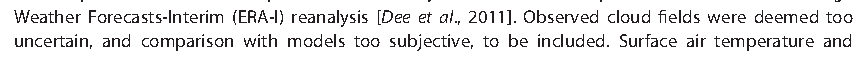
\includegraphics[width=0.7\linewidth]{./Figs/Pdf/tbert_text.pdf}
\end{center}
\end{frame}

\begin{frame}[label={sec:orgb9cda81}]{Pdf/tberth\_title.pdf}
\begin{center}
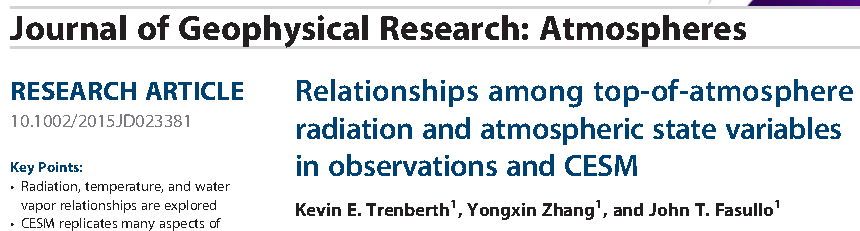
\includegraphics[width=0.7\linewidth]{./Figs/Pdf/tberth_title.pdf}
\end{center}
\end{frame}


\begin{frame}[label={sec:orgda91197}]{Png/rand\_global\_trend\_l1c\_vs\_era\_clr\_only\_fit\_chans.png}
\begin{center}
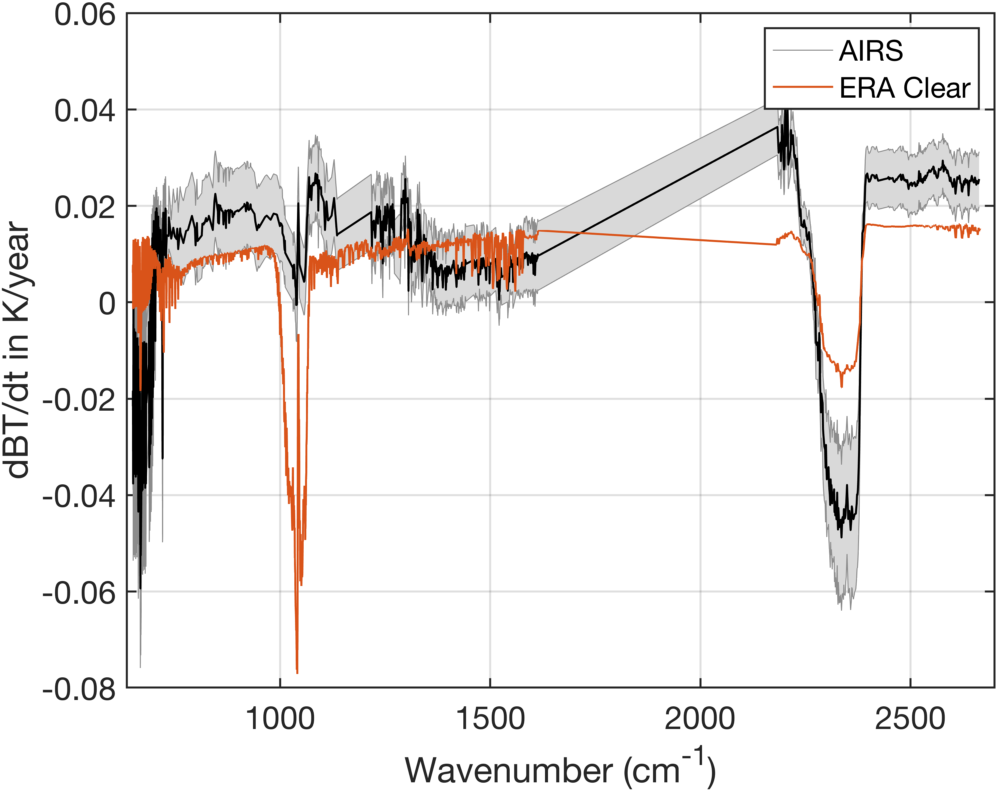
\includegraphics[width=0.7\linewidth]{./Figs/Png/rand_global_trend_l1c_vs_era_clr_only_fit_chans.png}
\end{center}
\end{frame}

\begin{frame}[label={sec:org0463493}]{Pdf/rand\_global\_trend\_l1c\_vs\_era\_clr.pdf}
\begin{center}
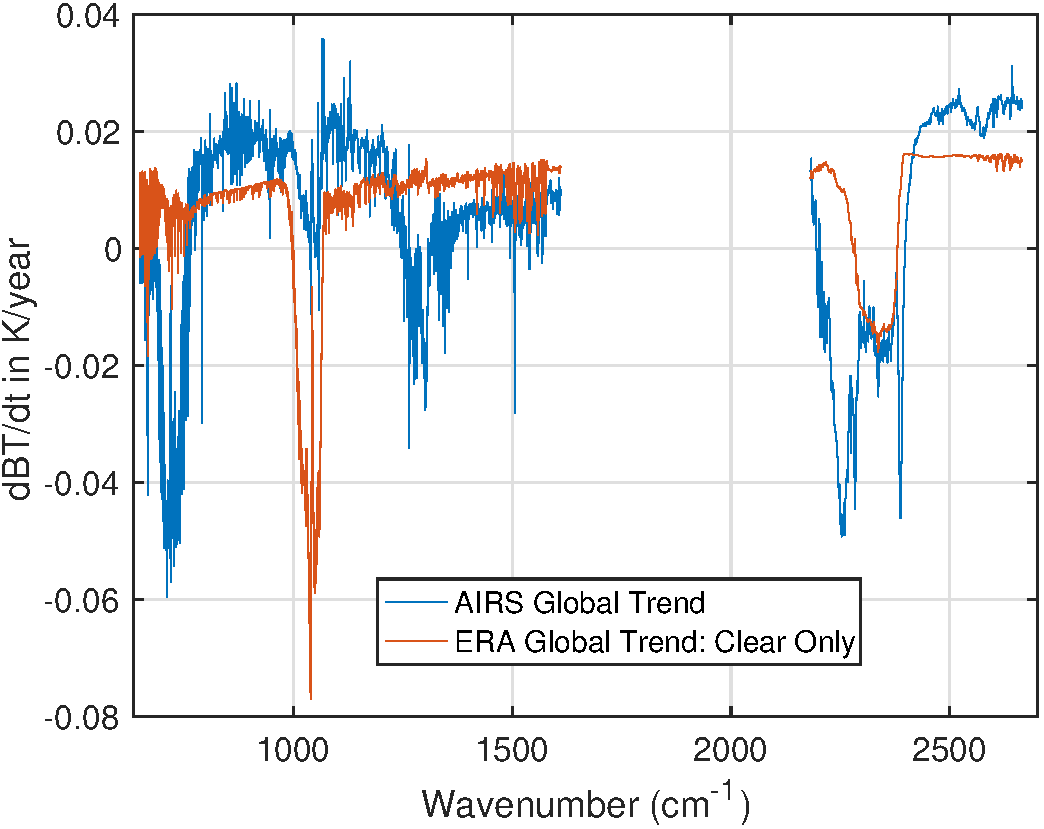
\includegraphics[width=0.7\linewidth]{./Figs/Pdf/rand_global_trend_l1c_vs_era_clr.pdf}
\end{center}
\end{frame}

\begin{frame}[label={sec:org398be72}]{Pdf/rand\_global\_trend\_l1c\_overview\_calfit\_marked.pdf}
\begin{center}
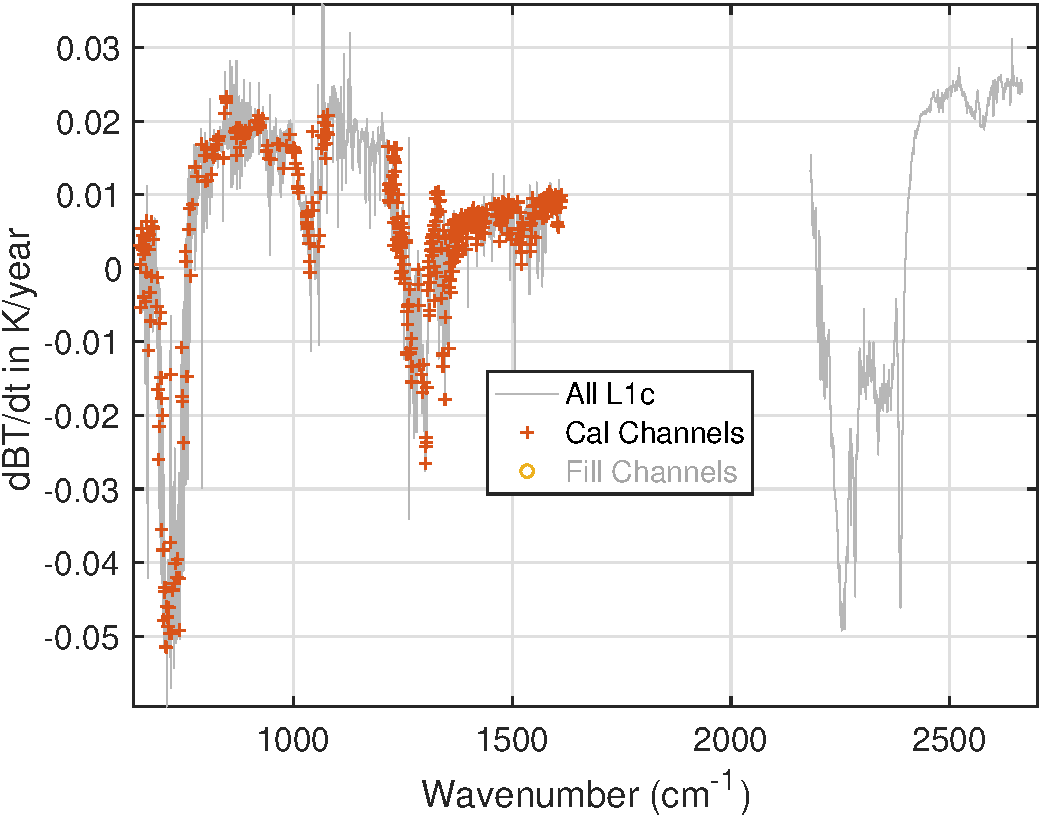
\includegraphics[width=0.7\linewidth]{./Figs/Pdf/rand_global_trend_l1c_overview_calfit_marked.pdf}
\end{center}
\end{frame}

\begin{frame}[label={sec:org24b6a71}]{Pdf/rand\_global\_trend\_l1c\_overview\_fill\_marked.pdf}
\begin{center}
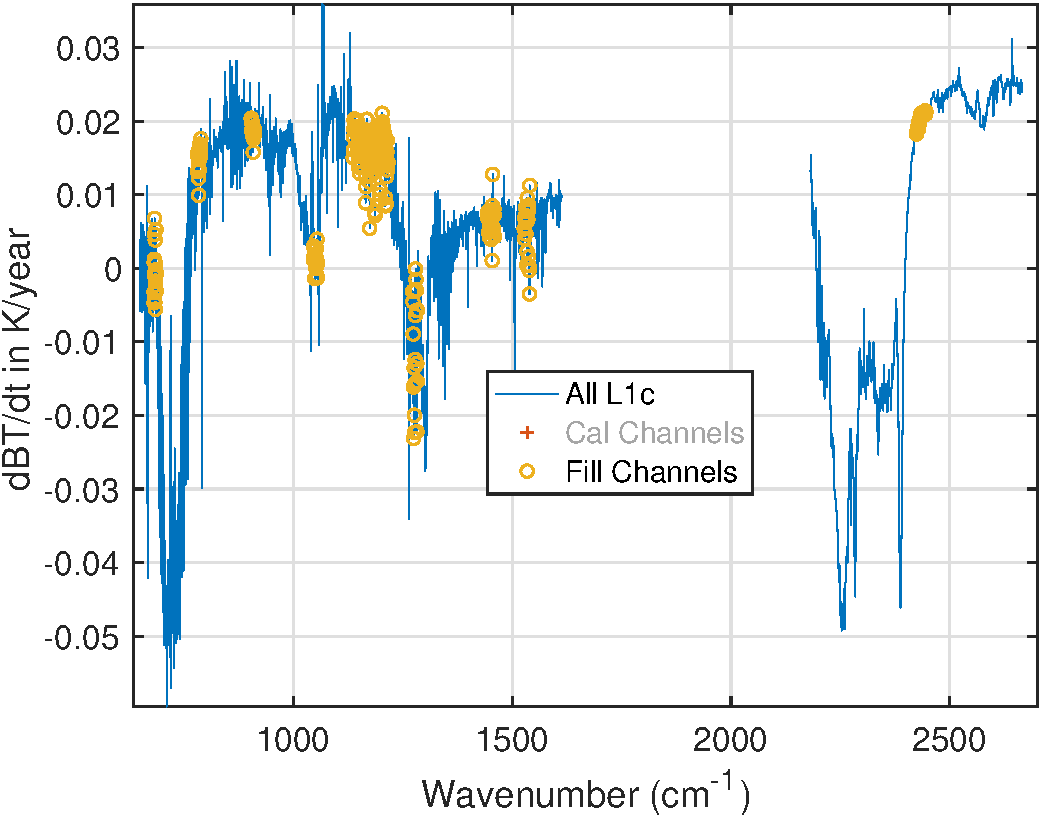
\includegraphics[width=0.7\linewidth]{./Figs/Pdf/rand_global_trend_l1c_overview_fill_marked.pdf}
\end{center}
\end{frame}

\begin{frame}[label={sec:orge2e4323}]{Pdf/rand\_global\_trend\_l1c\_overview.pdf}
\begin{center}
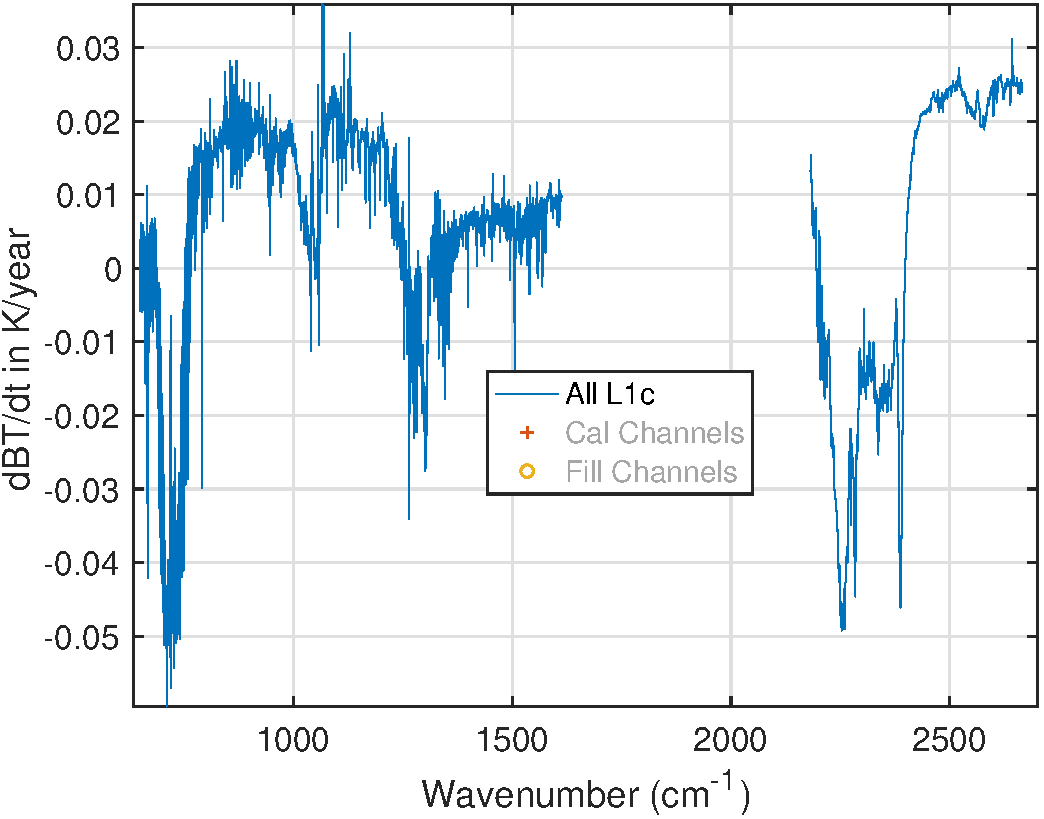
\includegraphics[width=0.7\linewidth]{./Figs/Pdf/rand_global_trend_l1c_overview.pdf}
\end{center}
\end{frame}




\begin{frame}[label={sec:org18c05b1}]{Pdf/raw\_co2\_vs\_era\_co2\_example\_lati28\_mlo\_lat.pdf}
\begin{center}
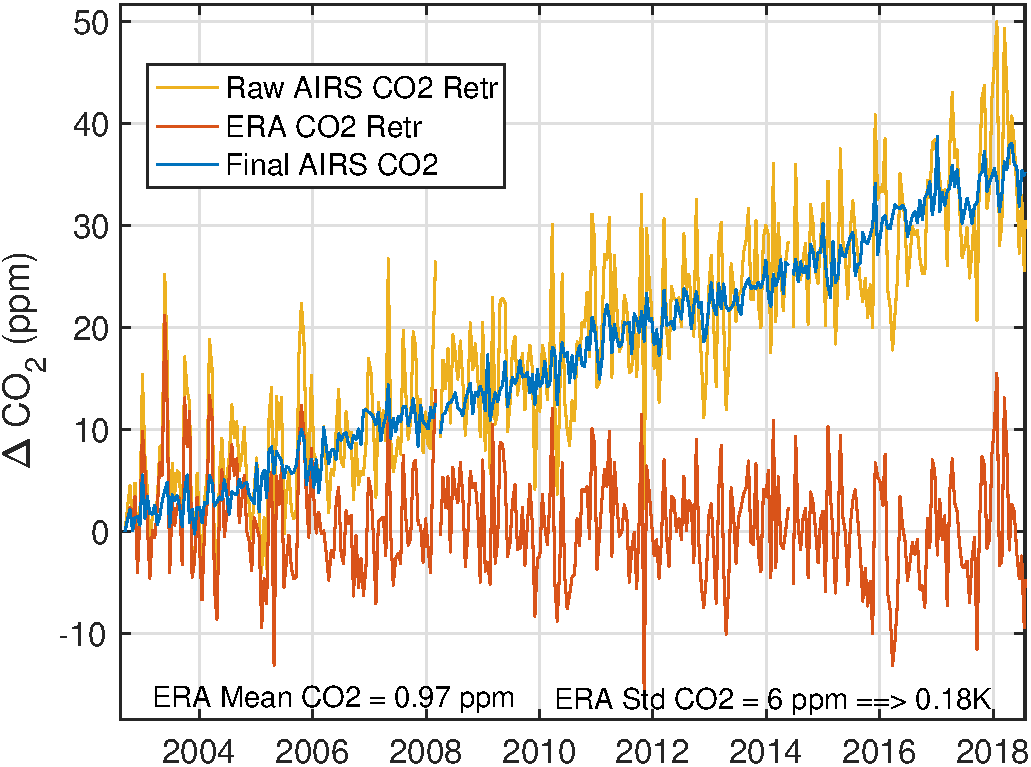
\includegraphics[width=0.7\linewidth]{./Figs/Pdf/raw_co2_vs_era_co2_example_lati28_mlo_lat.pdf}
\end{center}
\end{frame}

\begin{frame}[label={sec:org9eb2e65}]{Pdf/ch4\_airs\_vs\_esrl\_global\_growth\_anom.pdf}
\begin{center}
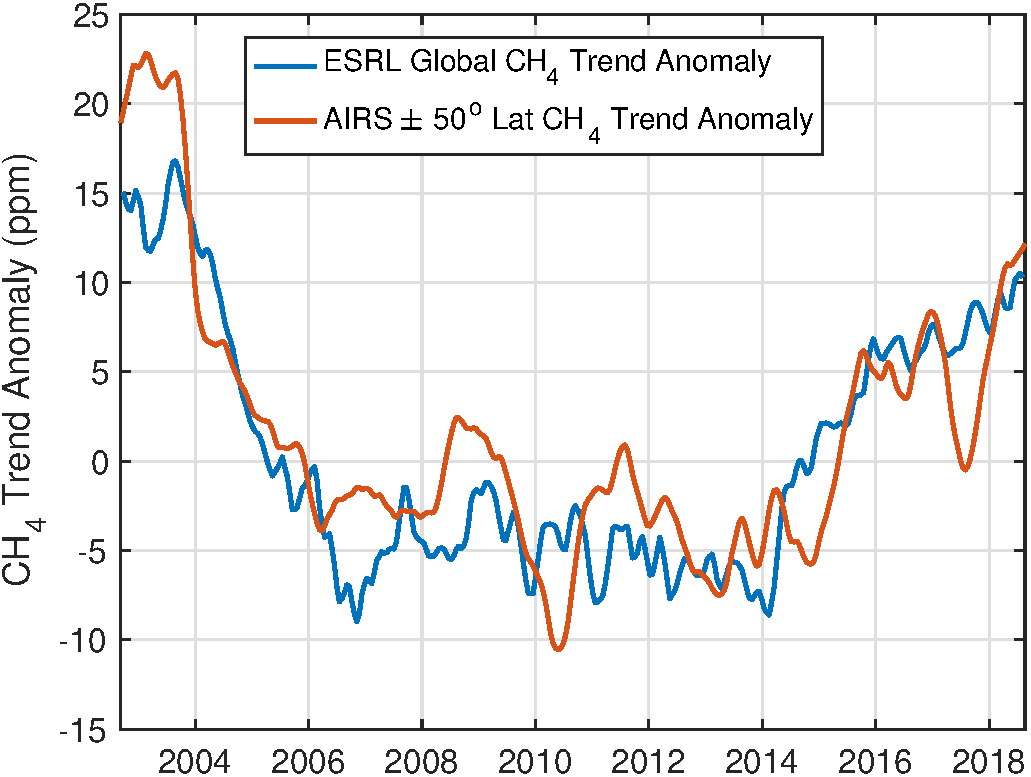
\includegraphics[width=0.7\linewidth]{./Figs/Pdf/ch4_airs_vs_esrl_global_growth_anom.pdf}
\end{center}
\end{frame}

\begin{frame}[label={sec:org52cd834}]{Pdf/ch4\_airs\_vs\_esrl\_global\_with\_dbt.pdf}
\begin{center}
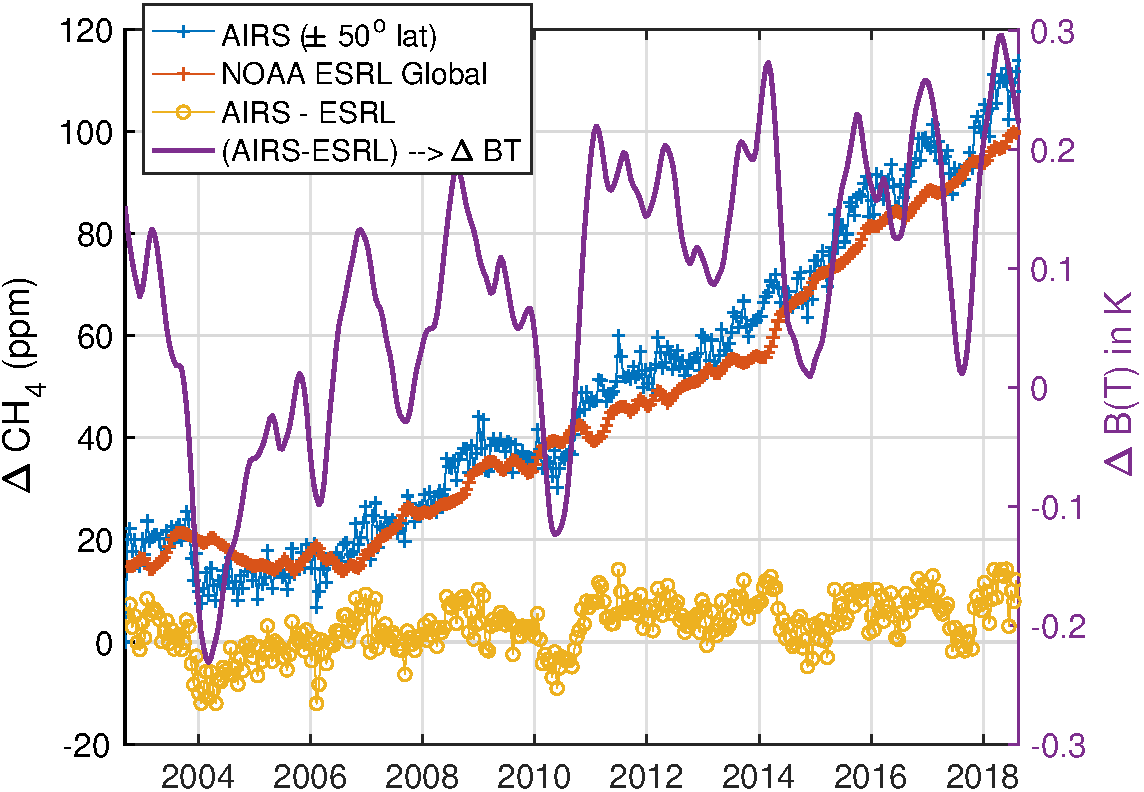
\includegraphics[width=0.7\linewidth]{./Figs/Pdf/ch4_airs_vs_esrl_global_with_dbt.pdf}
\end{center}
\end{frame}

\begin{frame}[label={sec:orgc3e65a7}]{Pdf/n2o\_airs\_vs\_esrl\_global\_with\_dbt.pdf}
\begin{center}
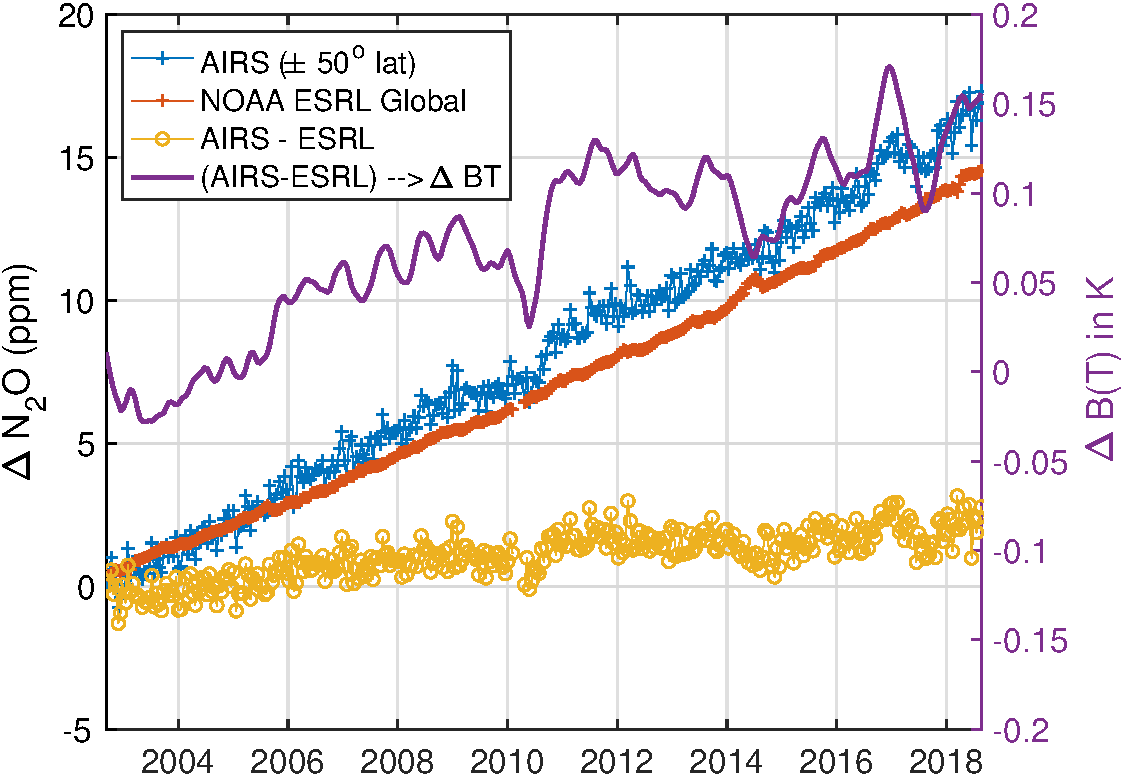
\includegraphics[width=0.7\linewidth]{./Figs/Pdf/n2o_airs_vs_esrl_global_with_dbt.pdf}
\end{center}
\end{frame}

\begin{frame}[label={sec:org5422f83}]{Png/co2\_anomaly\_image\_fancy2\_corrected.png}
\begin{center}
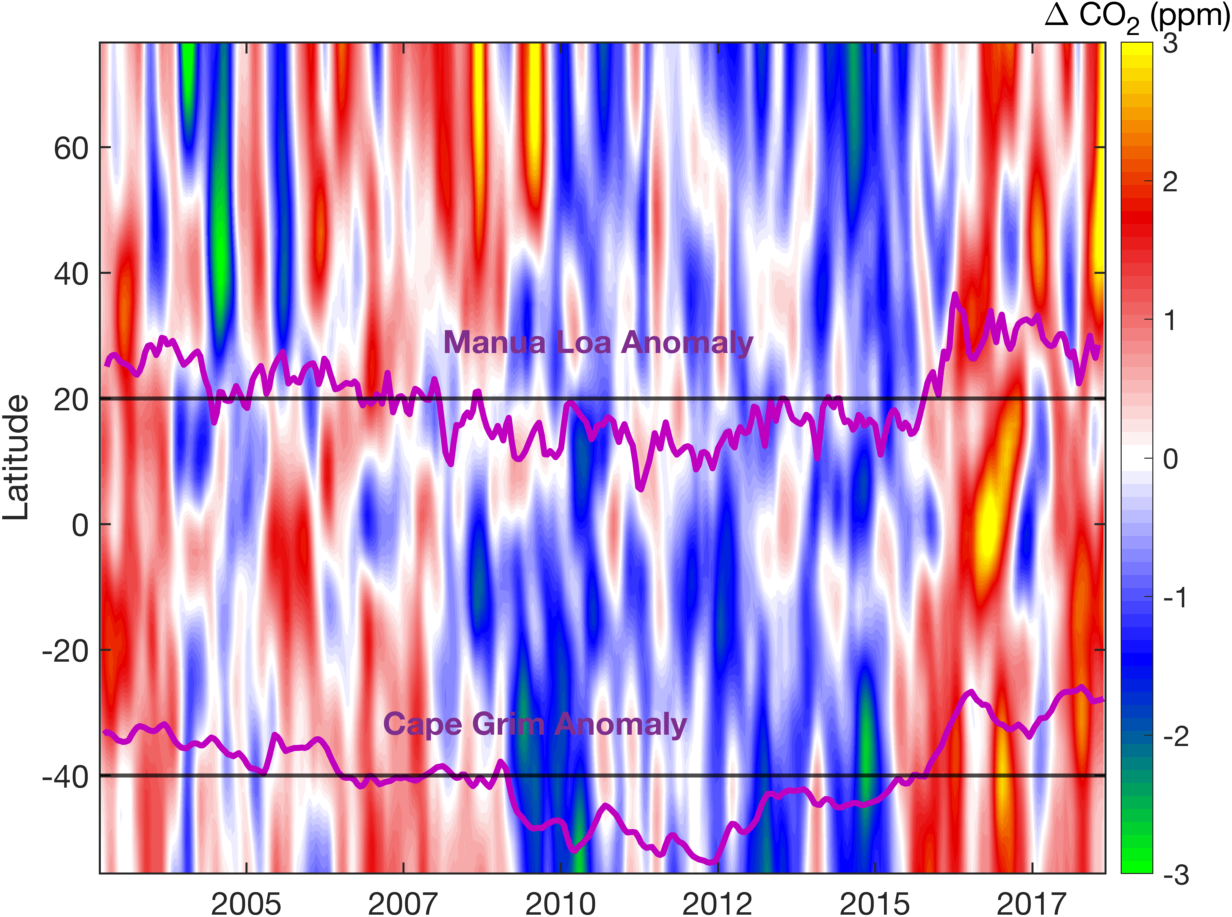
\includegraphics[width=0.7\linewidth]{./Figs/Png/co2_anomaly_image_fancy2_corrected.png}
\end{center}
\end{frame}

\begin{frame}[label={sec:orgff22418}]{Png/co2\_anom\_image\_lat\_vs\_time.png}
\begin{center}
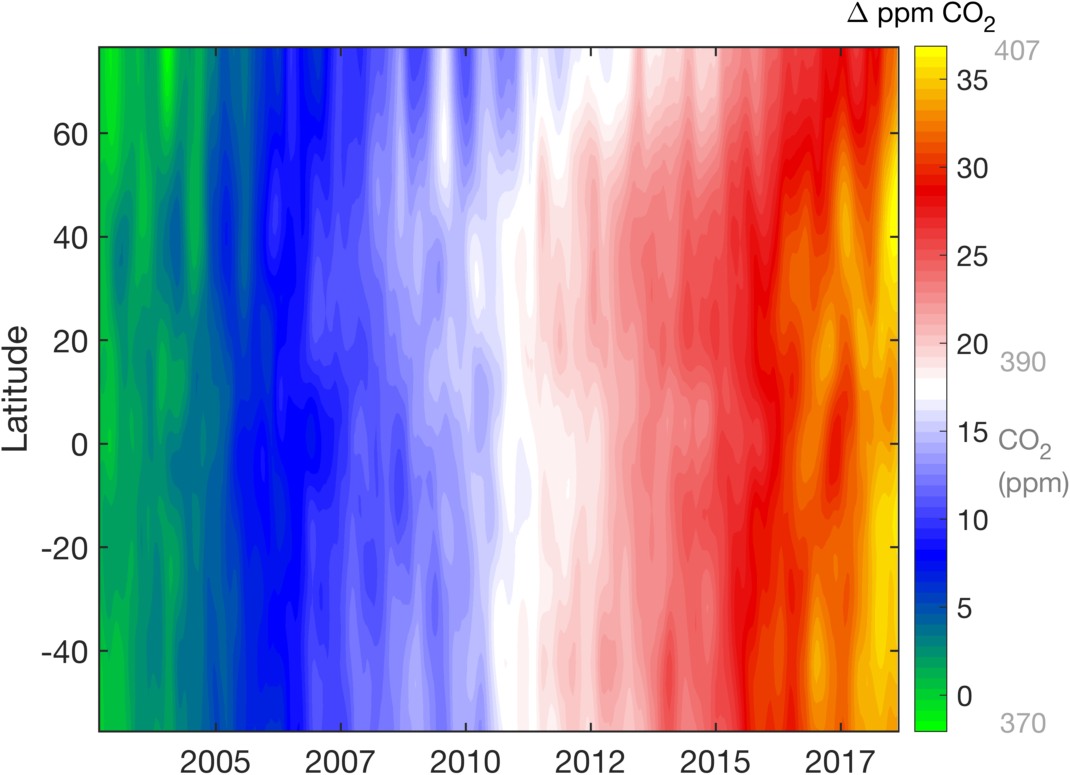
\includegraphics[width=0.7\linewidth]{./Figs/Png/co2_anom_image_lat_vs_time.png}
\end{center}
\end{frame}

\begin{frame}[label={sec:org29a70c6}]{Pdf/co2\_airs\_vs\_esrl\_global\_growth\_anom.pdf}
\begin{center}
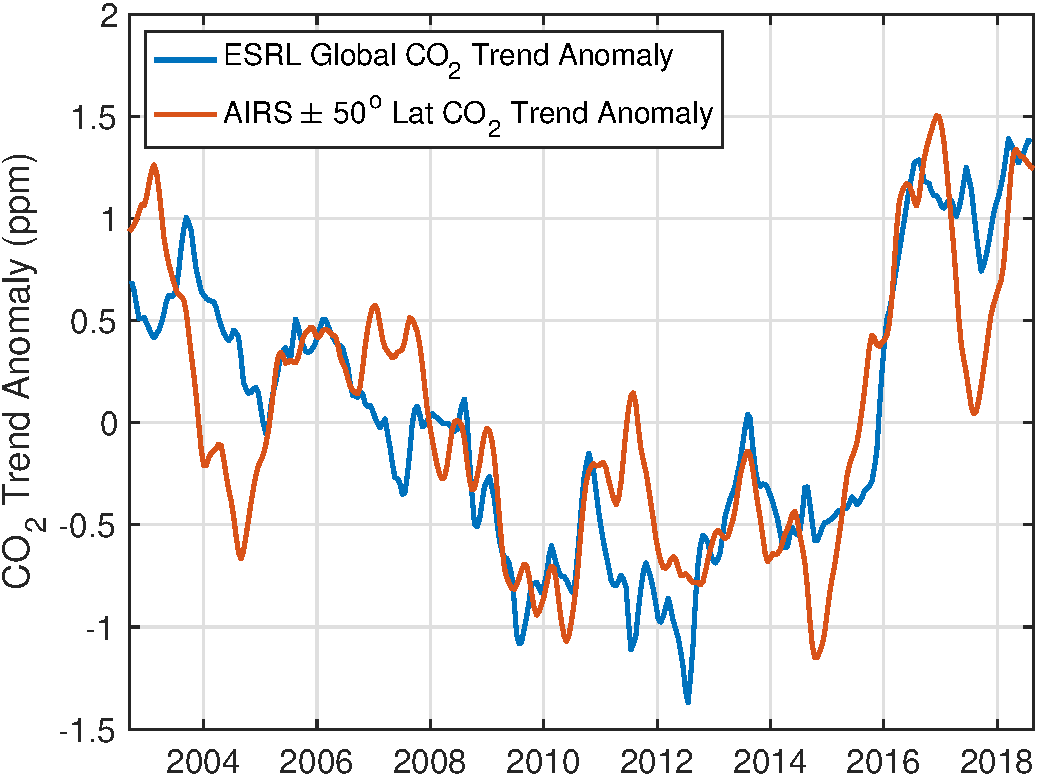
\includegraphics[width=0.7\linewidth]{./Figs/Pdf/co2_airs_vs_esrl_global_growth_anom.pdf}
\end{center}
\end{frame}

\begin{frame}[label={sec:org94b7c72}]{Pdf/co2\_airs\_vs\_mlo.pdf}
\begin{center}
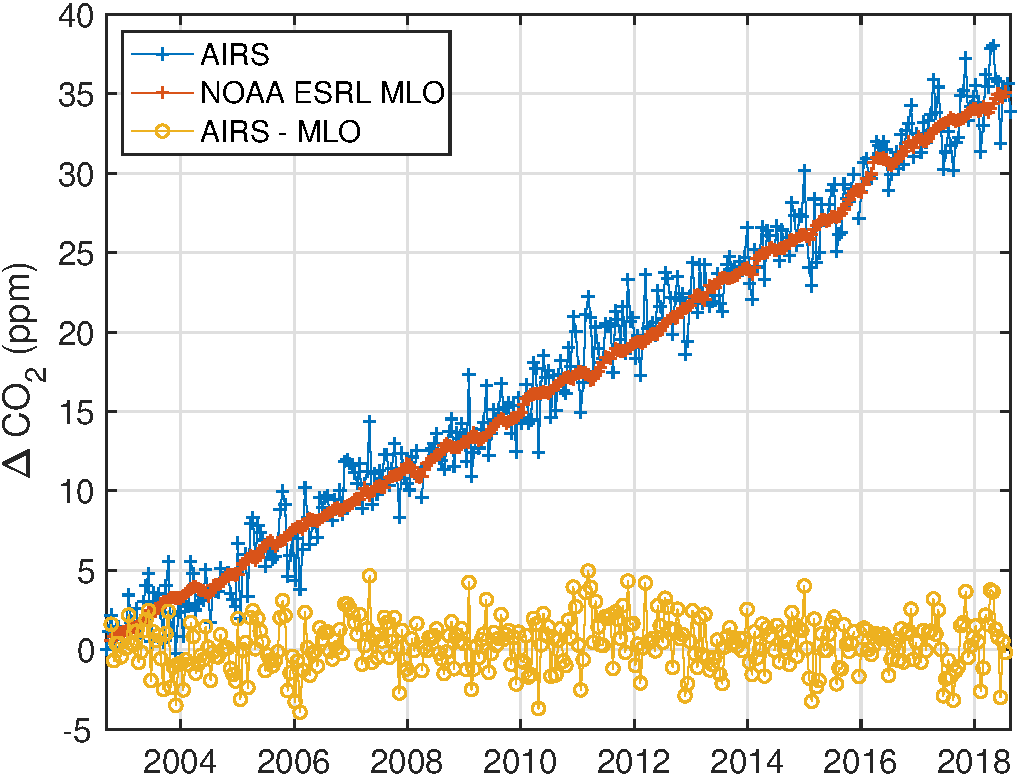
\includegraphics[width=0.7\linewidth]{./Figs/Pdf/co2_airs_vs_mlo.pdf}
\end{center}
\end{frame}

\begin{frame}[label={sec:orgaf32f3e}]{Pdf/co2\_airs\_vs\_esrl\_global\_with\_dbt.pdf}
\begin{center}
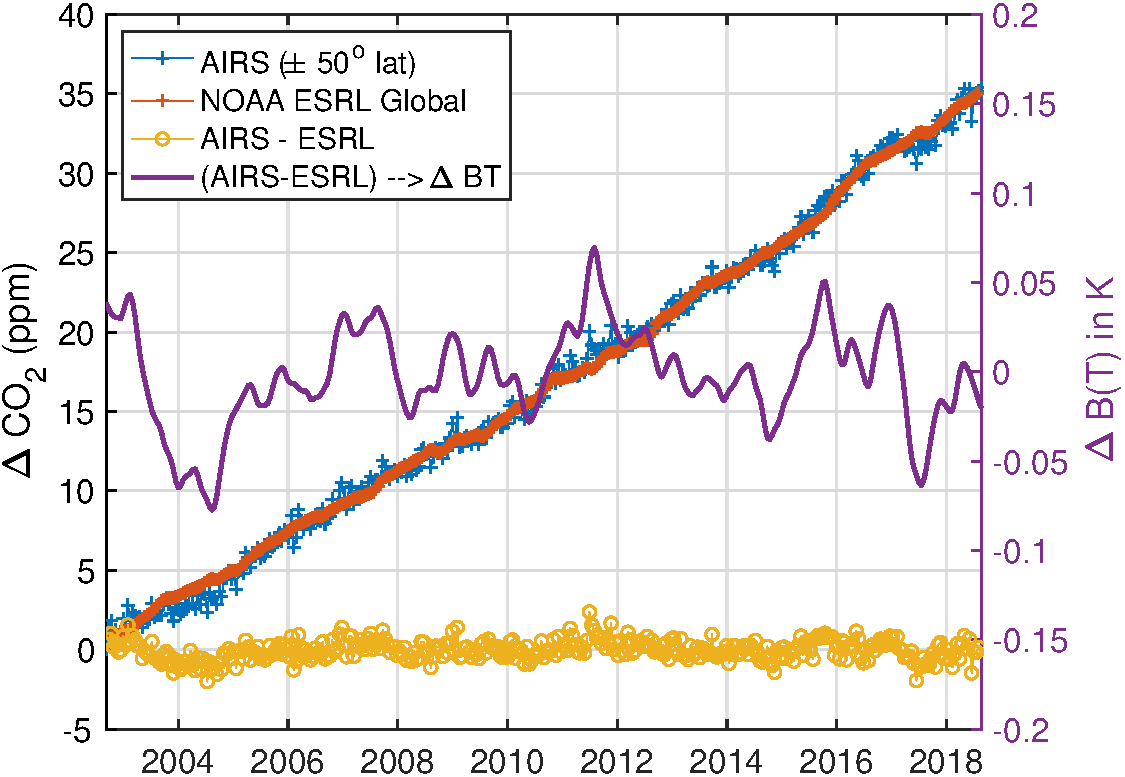
\includegraphics[width=0.7\linewidth]{./Figs/Pdf/co2_airs_vs_esrl_global_with_dbt.pdf}
\end{center}
\end{frame}

\begin{frame}[label={sec:org1d4f9d6}]{Pdf/co2\_growth\_vs\_lat.pdf}
\begin{center}
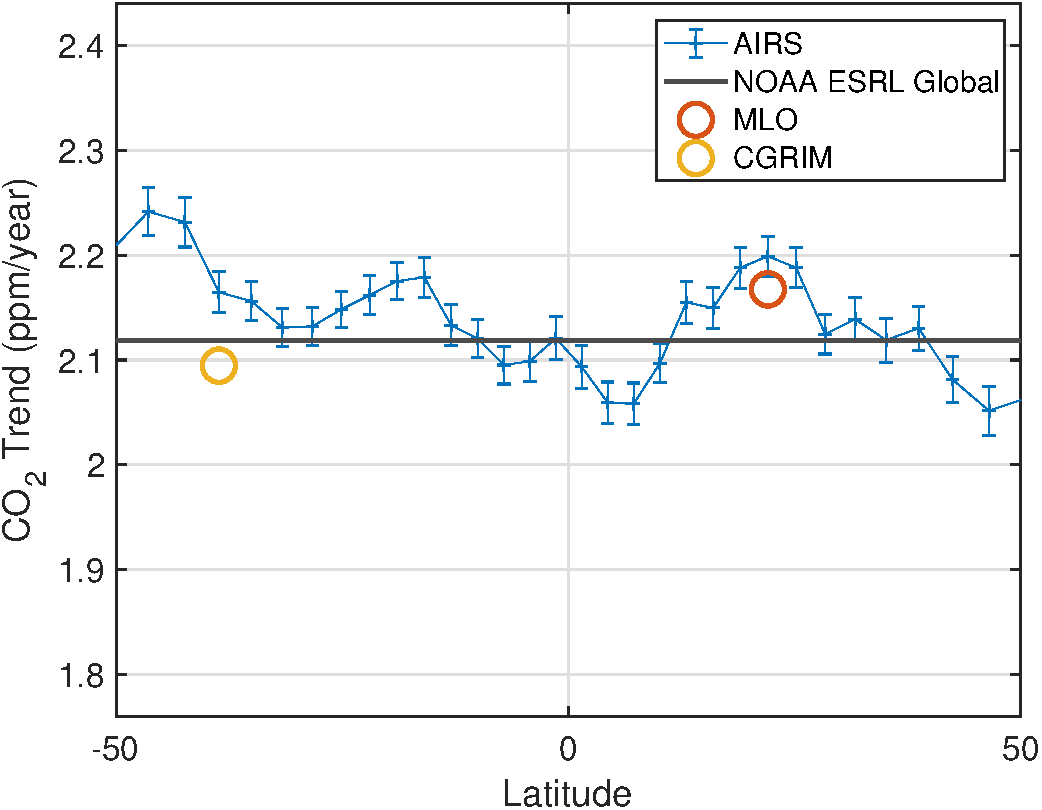
\includegraphics[width=0.7\linewidth]{./Figs/Pdf/co2_growth_vs_lat.pdf}
\end{center}
\end{frame}

\begin{frame}[label={sec:orgf82945e}]{Png/best\_co2\_anomaly\_resid\_fit\_chans\_concat.png}
\begin{center}
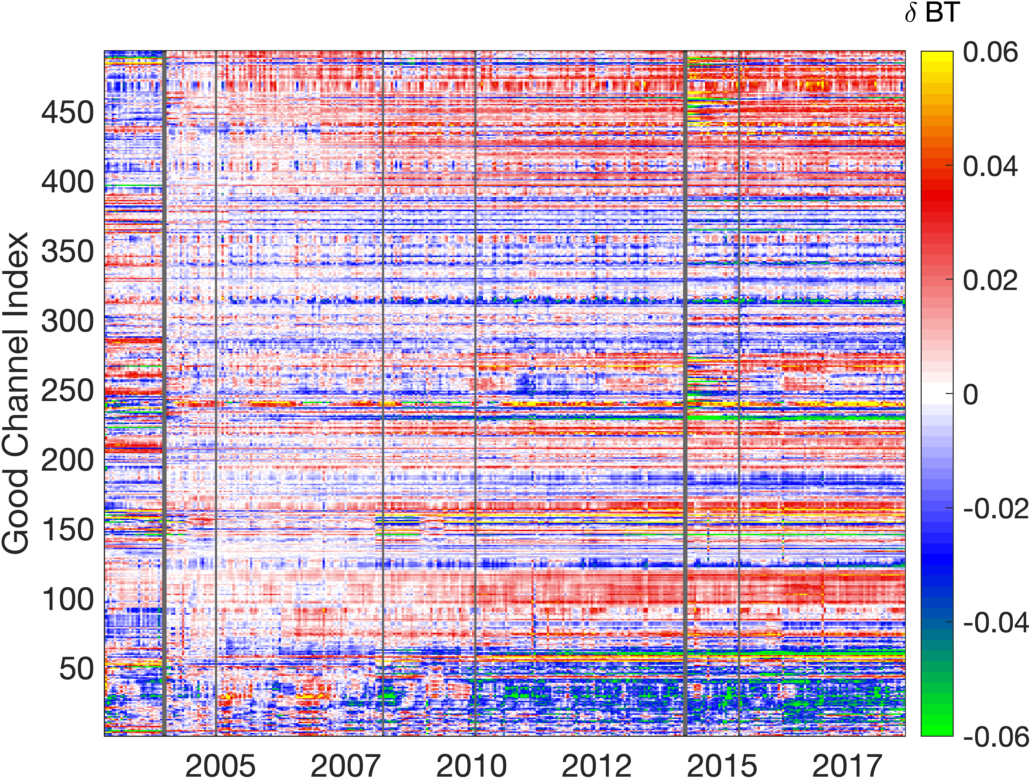
\includegraphics[width=0.7\linewidth]{./Figs/Png/best_co2_anomaly_resid_fit_chans_concat.png}
\end{center}
\end{frame}

\begin{frame}[label={sec:org8e52b0b}]{Png/best\_co2\_anomaly\_resid\_fit\_chans.png}
\begin{center}
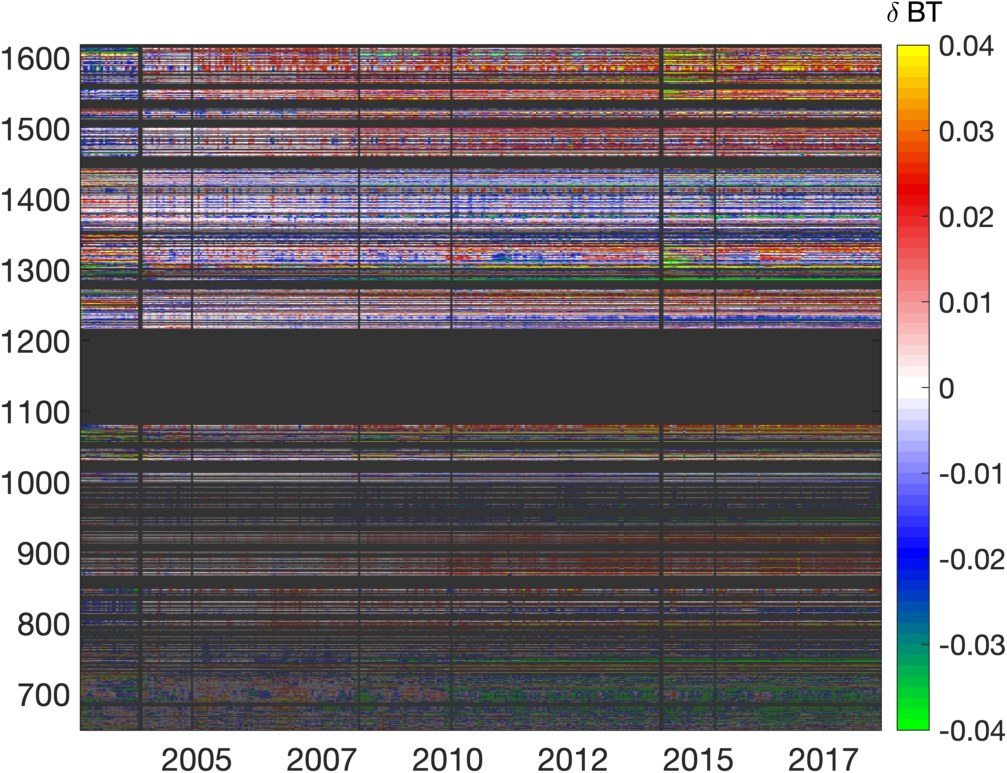
\includegraphics[width=0.7\linewidth]{./Figs/Png/best_co2_anomaly_resid_fit_chans.png}
\end{center}
\end{frame}

\begin{frame}[label={sec:org8435298}]{Png/best\_co2\_anom\_resid\_no\_sw.png}
\begin{center}
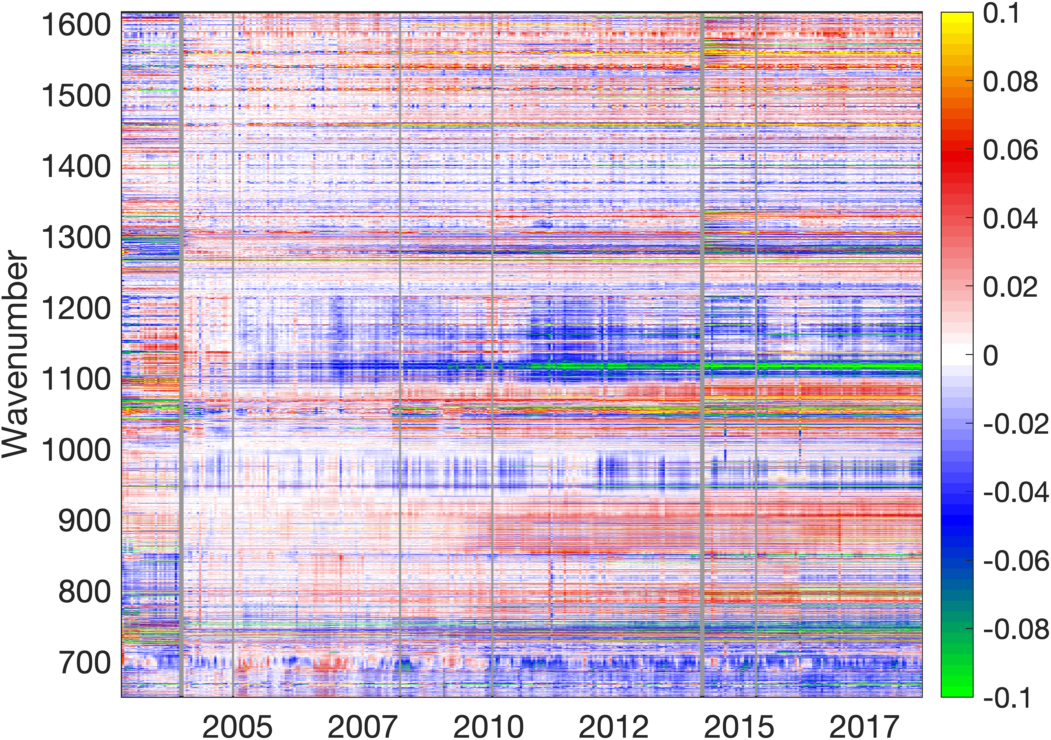
\includegraphics[width=0.7\linewidth]{./Figs/Png/best_co2_anom_resid_no_sw.png}
\end{center}
\end{frame}

\begin{frame}[label={sec:org7bf95d1}]{Png/best\_co2\_anom\_resid.png}
\begin{center}
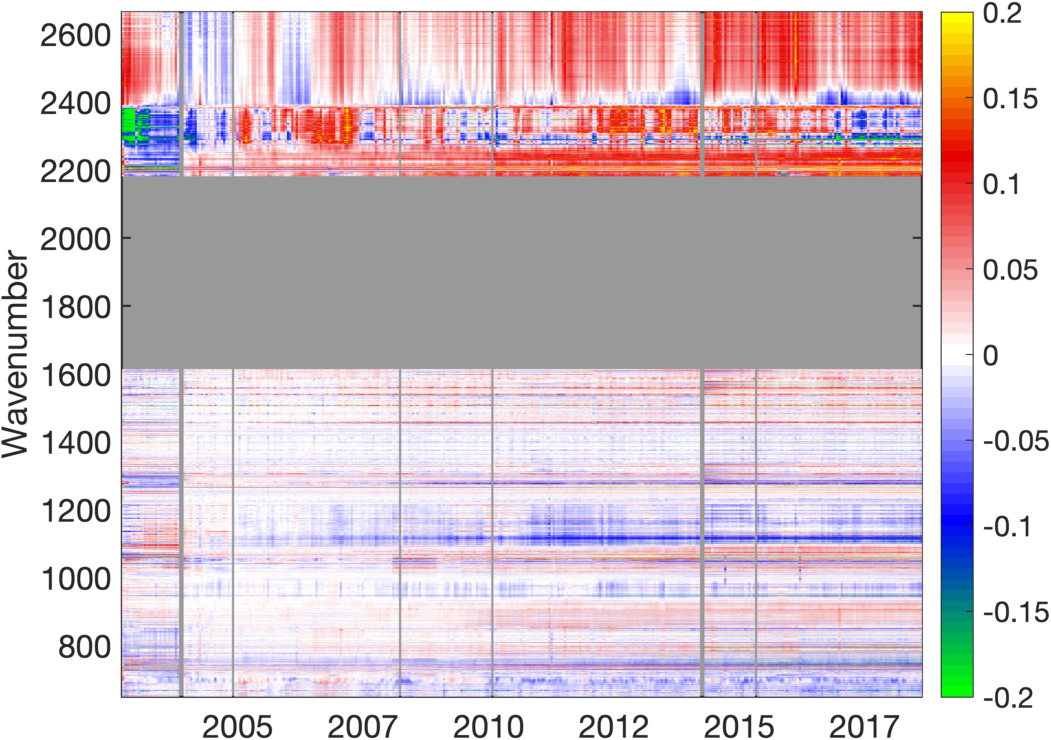
\includegraphics[width=0.7\linewidth]{./Figs/Png/best_co2_anom_resid.png}
\end{center}
\end{frame}

\begin{frame}[label={sec:orgbf7072d}]{Pdf/airs\_cfc\_bias\_iasi\_times.pdf}
\begin{center}
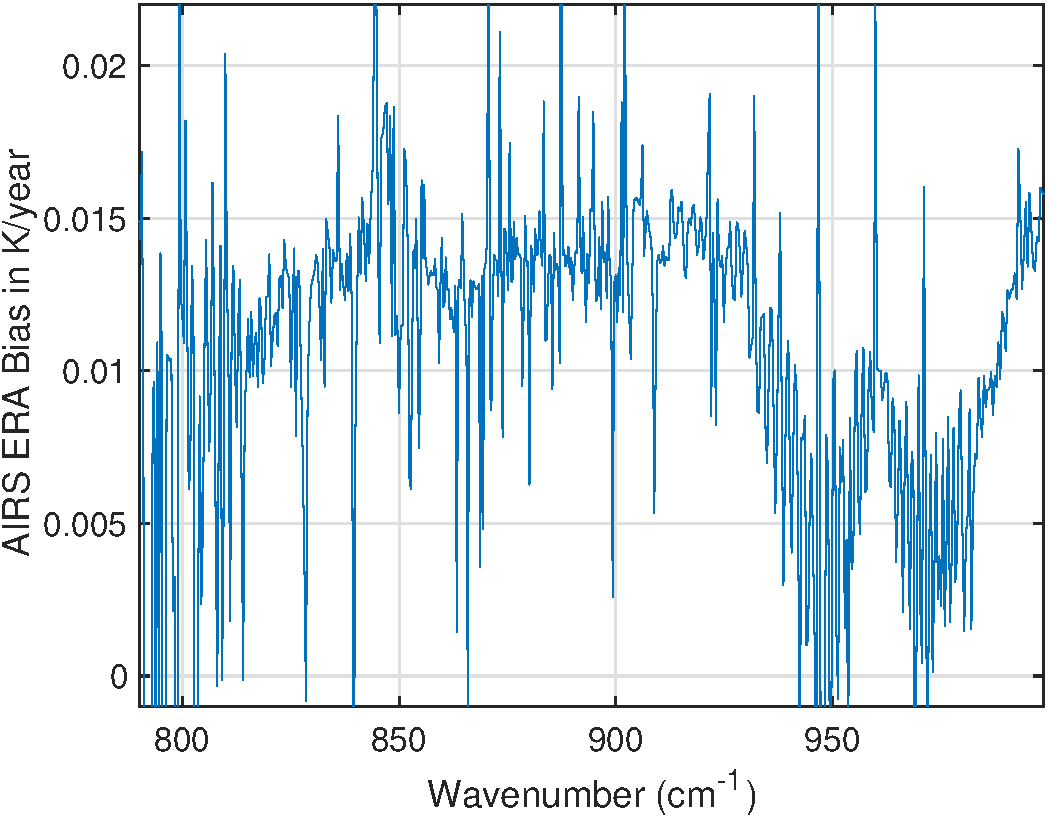
\includegraphics[width=0.7\linewidth]{./Figs/Pdf/airs_cfc_bias_iasi_times.pdf}
\end{center}
\end{frame}

\begin{frame}[label={sec:org7d67f19}]{Pdf/cfc11\_bt\_trend.pdf}
\begin{center}
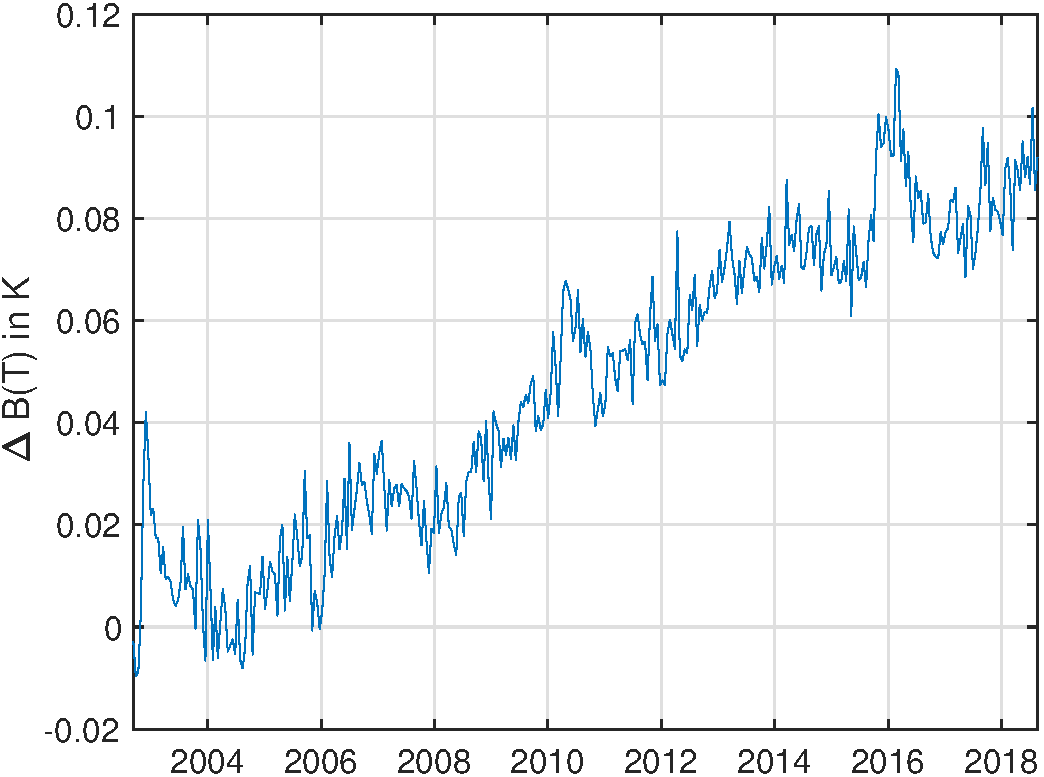
\includegraphics[width=0.7\linewidth]{./Figs/Pdf/cfc11_bt_trend.pdf}
\end{center}
\end{frame}

\begin{frame}[label={sec:org0843af6}]{Pdf/cfc11\_trend.pdf}
\begin{center}
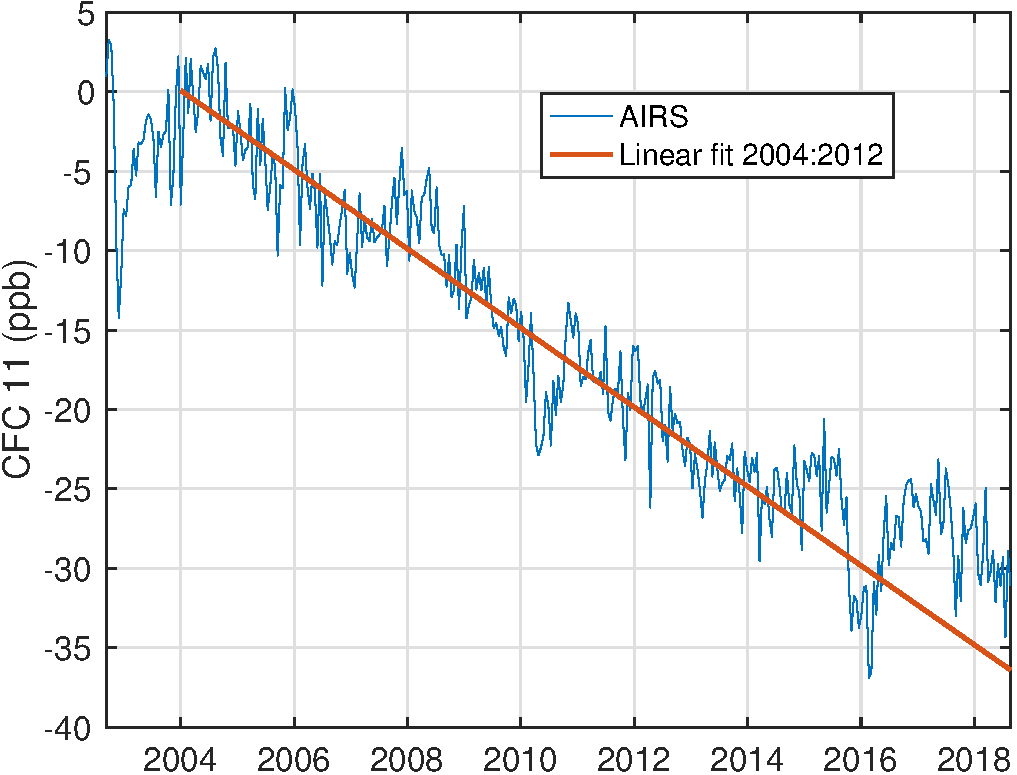
\includegraphics[width=0.7\linewidth]{./Figs/Pdf/cfc11_trend.pdf}
\end{center}
\end{frame}

\begin{frame}[label={sec:org6fab763}]{Pdf/co2\_anom\_sst\_vs\_oisst\_clear\_sampled\_and\_era.pdf}
\begin{center}
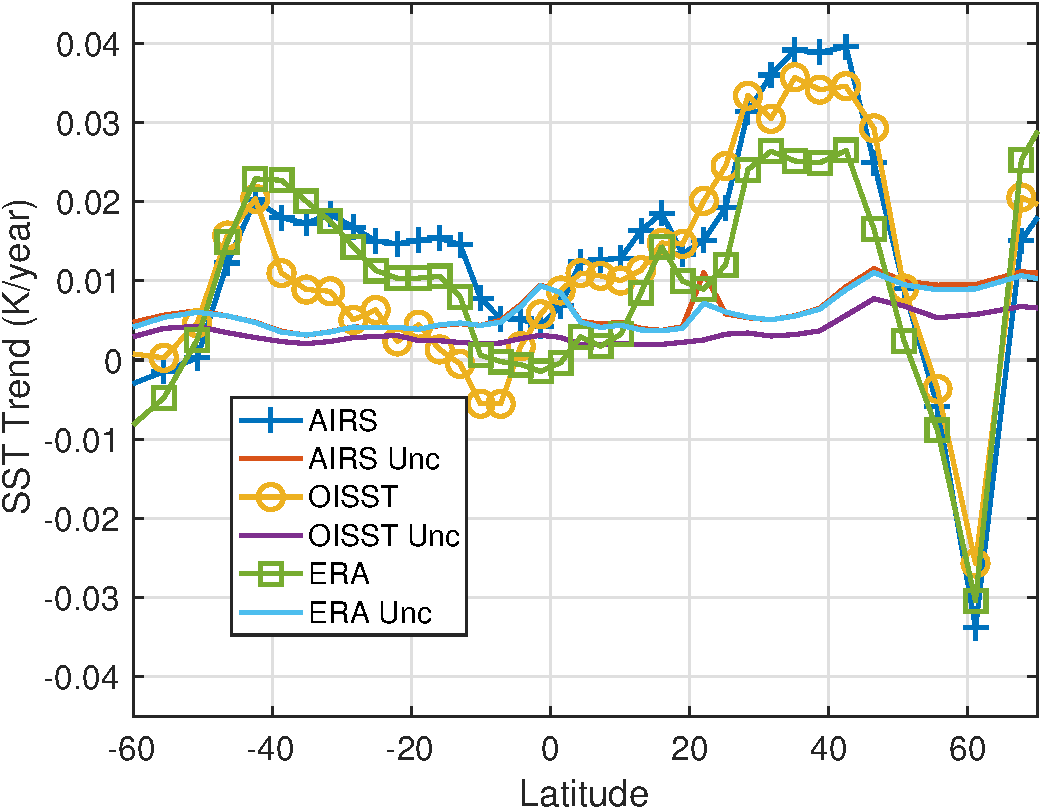
\includegraphics[width=0.7\linewidth]{./Figs/Pdf/co2_anom_sst_vs_oisst_clear_sampled_and_era.pdf}
\end{center}
\end{frame}

\begin{frame}[label={sec:org0d5ade3}]{Pdf/co2\_anom\_sst\_vs\_oisst\_clear\_sampled.pdf}
\begin{center}
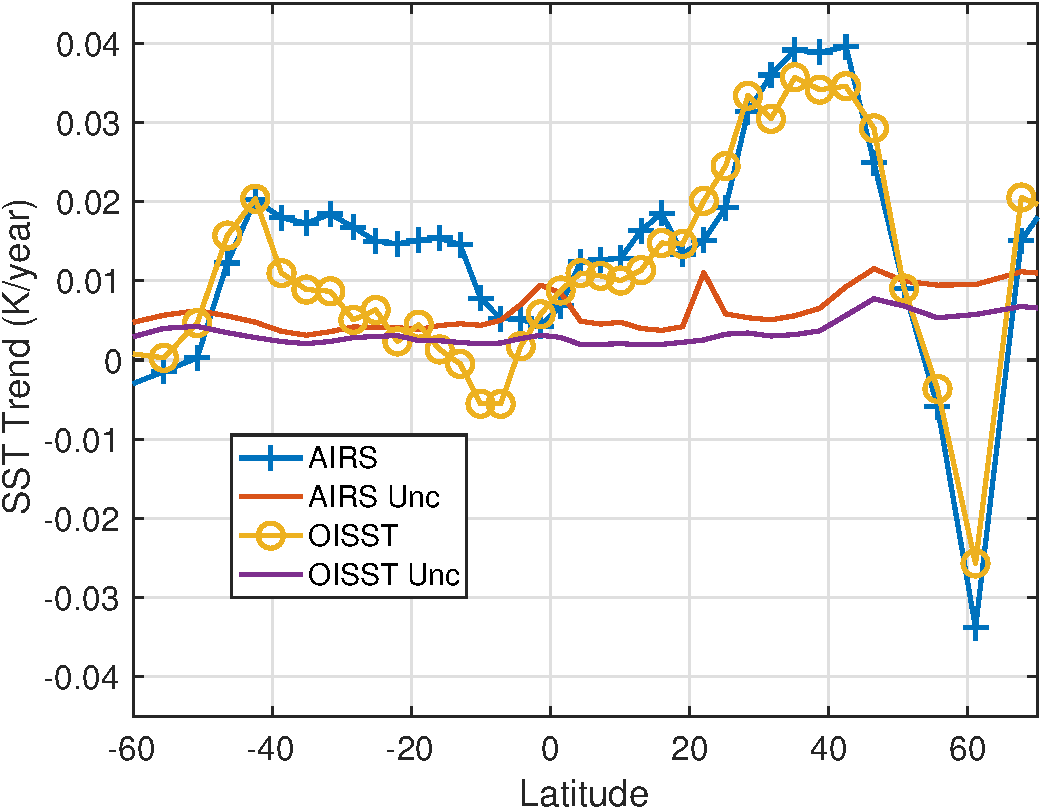
\includegraphics[width=0.7\linewidth]{./Figs/Pdf/co2_anom_sst_vs_oisst_clear_sampled.pdf}
\end{center}
\end{frame}



\begin{frame}[label={sec:org6f90b9b}]{Pdf/resid\_spectrum\_dec17\_minus\_oct14\_2003\_swzoom.pdf}
\begin{center}
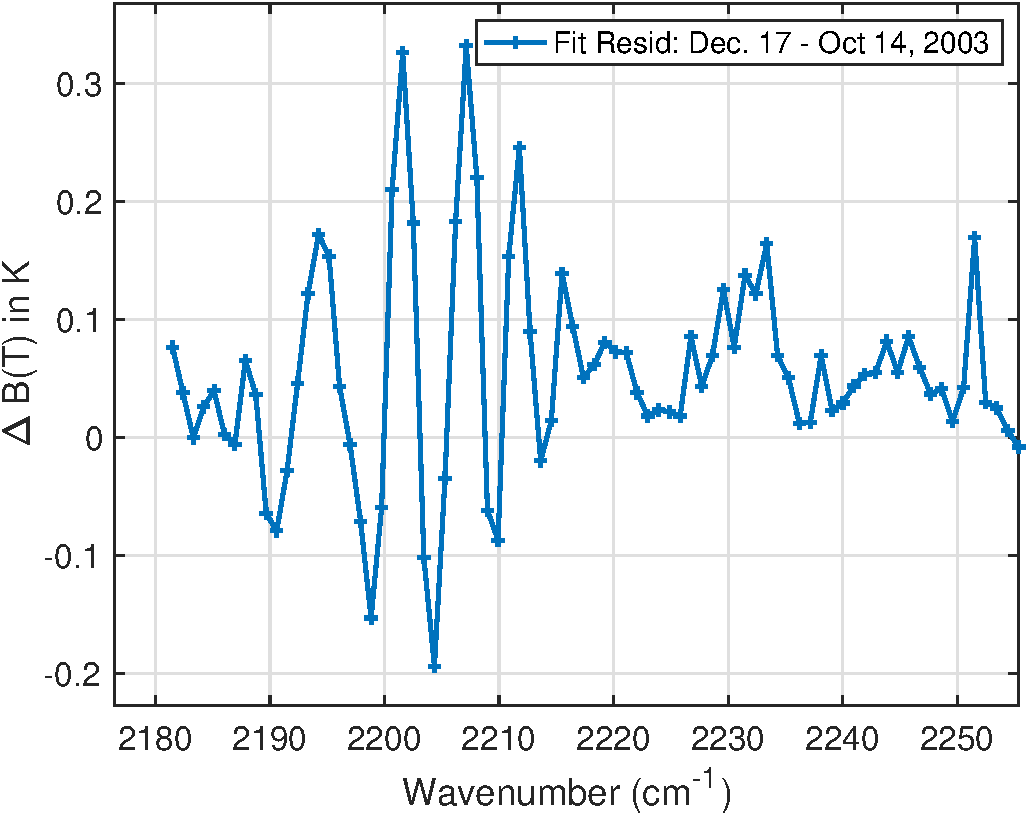
\includegraphics[width=0.7\linewidth]{./Figs/Pdf/resid_spectrum_dec17_minus_oct14_2003_swzoom.pdf}
\end{center}
\end{frame}

\begin{frame}[label={sec:org790fa7c}]{Pdf/resid\_spectrum\_dec17\_minus\_oct14\_2003.pdf}
\begin{center}
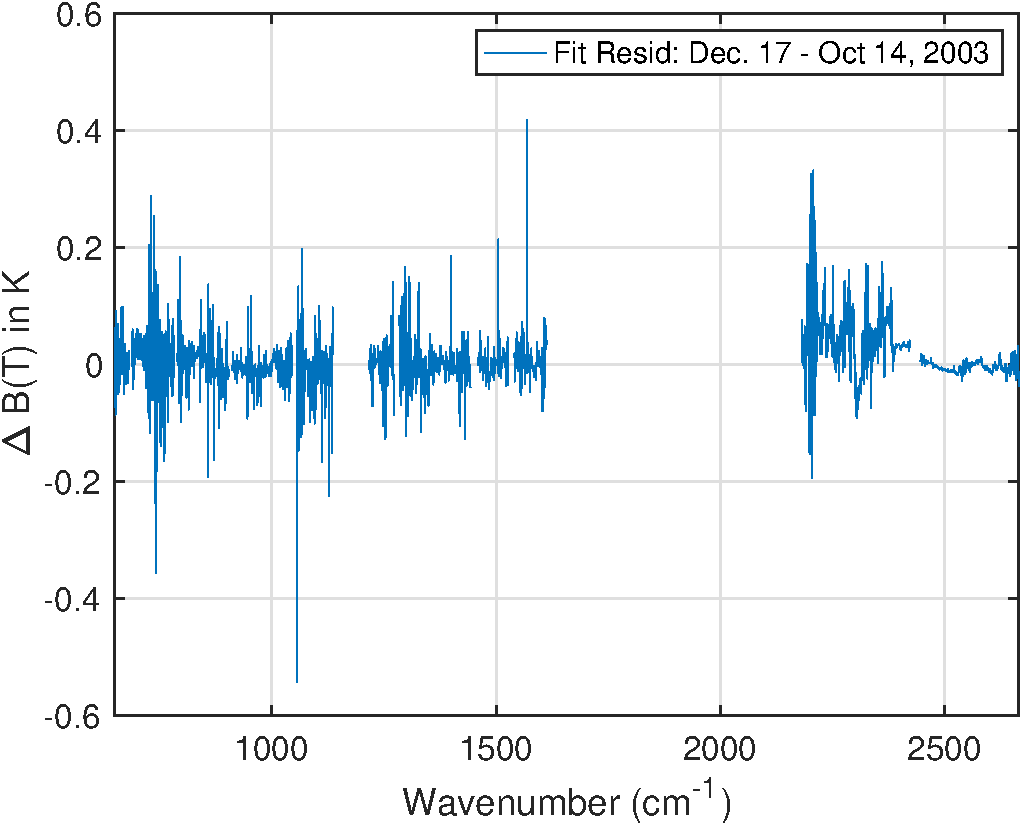
\includegraphics[width=0.7\linewidth]{./Figs/Pdf/resid_spectrum_dec17_minus_oct14_2003.pdf}
\end{center}
\end{frame}

\begin{frame}[label={sec:org2038cf0}]{Pdf/resid\_1567\_and\_1570\_cm01\_dnu.pdf}
\begin{center}
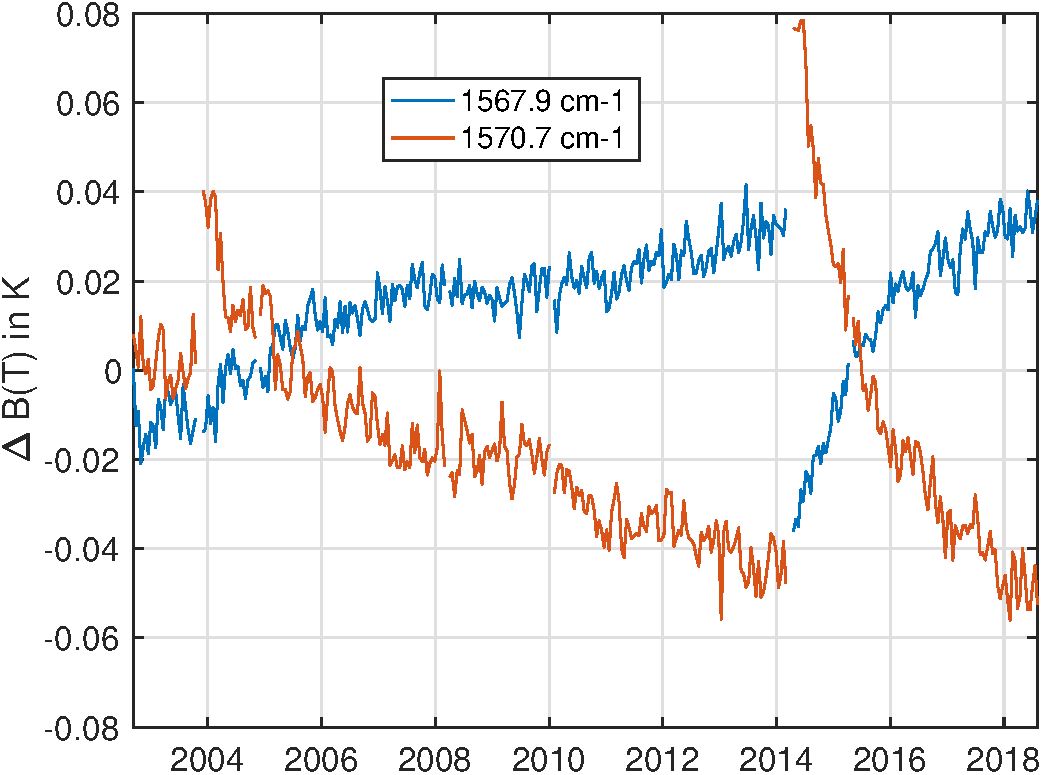
\includegraphics[width=0.7\linewidth]{./Figs/Pdf/resid_1567_and_1570_cm01_dnu.pdf}
\end{center}
\end{frame}

\begin{frame}[label={sec:org82970e8}]{Png/resid\_872to939cm-1\_drift\_and\_1471to1541.png}
\begin{center}
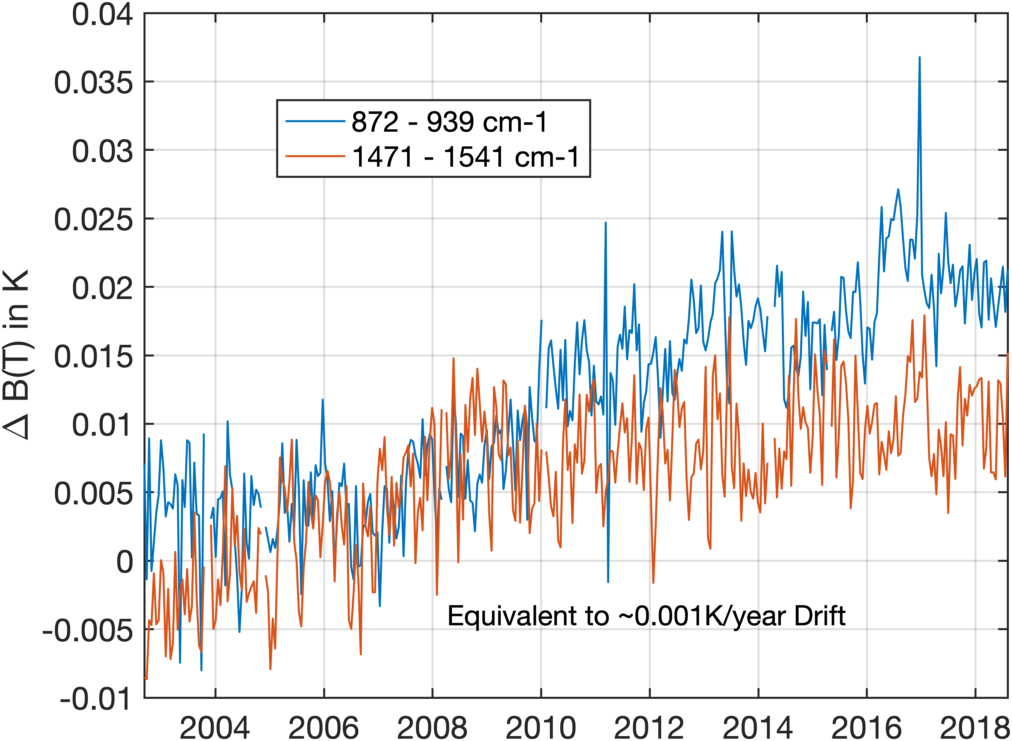
\includegraphics[width=0.7\linewidth]{./Figs/Png/resid_872to939cm-1_drift_and_1471to1541.png}
\end{center}
\end{frame}

\begin{frame}[label={sec:org0a0dc42}]{Pdf/resid\_872to939cm-1\_drift.pdf}
\begin{center}
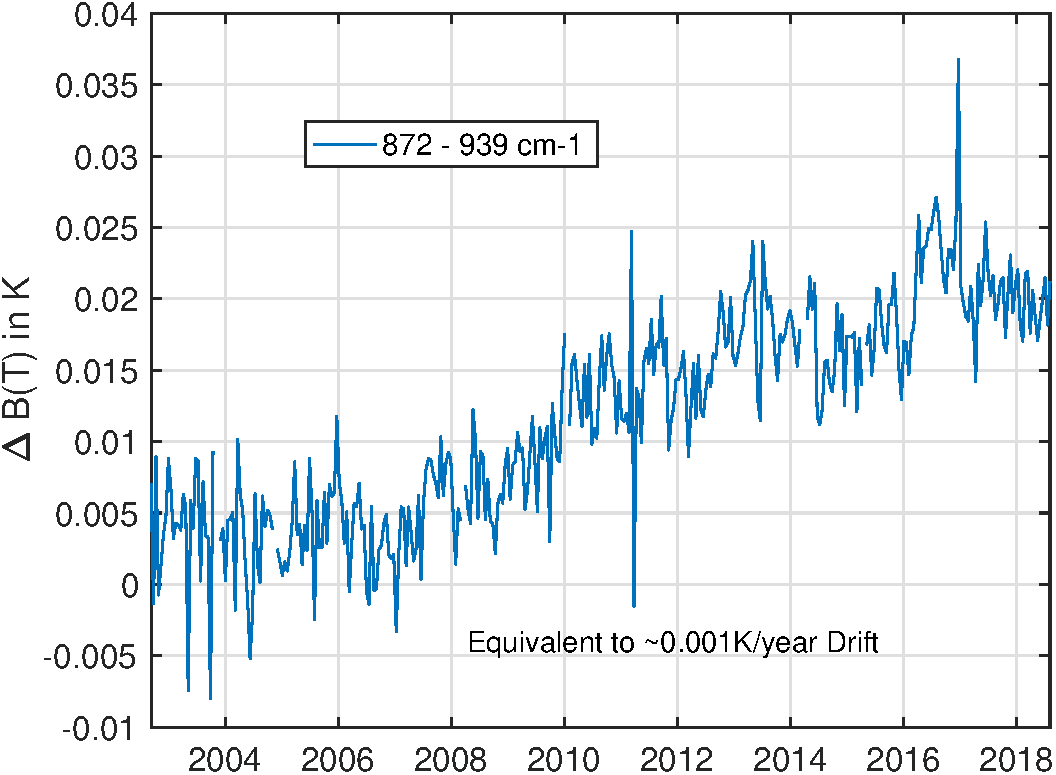
\includegraphics[width=0.7\linewidth]{./Figs/Pdf/resid_872to939cm-1_drift.pdf}
\end{center}
\end{frame}


\begin{frame}[label={sec:org41edc10}]{DCC1}
\begin{figure}[htbp]
\centering
\includegraphics[width=\linewidth]{./Figsdc/Pdf/bt2616_and_bt960_dcc_vs_time_airs_and_iasi.pdf}
\caption{\emph{AIRS and IASI Dcc daily average temperatures versus time.  The IASI curve for 2616 cm\textsuperscript{-1} is an average over 54 IASI channels.}}
\end{figure}
\end{frame}

\begin{frame}[label={sec:orgd9280c4}]{DCC4}
\begin{figure}[htbp]
\centering
\includegraphics[width=\linewidth]{./Figsdc/Pdf/airs_iasi_dcc_rate_sw_iasi_avgpts.pdf}
\caption{\emph{Same as Fig. where? with every two points in IASI averaged.}}
\end{figure}
\end{frame}

\begin{frame}[label={sec:org2a1f757}]{DCC6}
\begin{figure}[htbp]
\centering
\includegraphics[width=\linewidth]{./Figsdc/Pdf/airs_iasi_dcc_rate_lw_ab_diffs_vs_iasi.pdf}
\caption{\emph{Longwave DCC linear rate of change with AIRS A,B, AB channels identifications highlighted.}}
\end{figure}
\end{frame}



\begin{frame}[label={sec:org4cfc113}]{Pdf/zonal\_sst\_trends\_12311\_vs\_oisst\_ersst5\_hottest\_per\_grid\_envelope.pdf}
\begin{center}
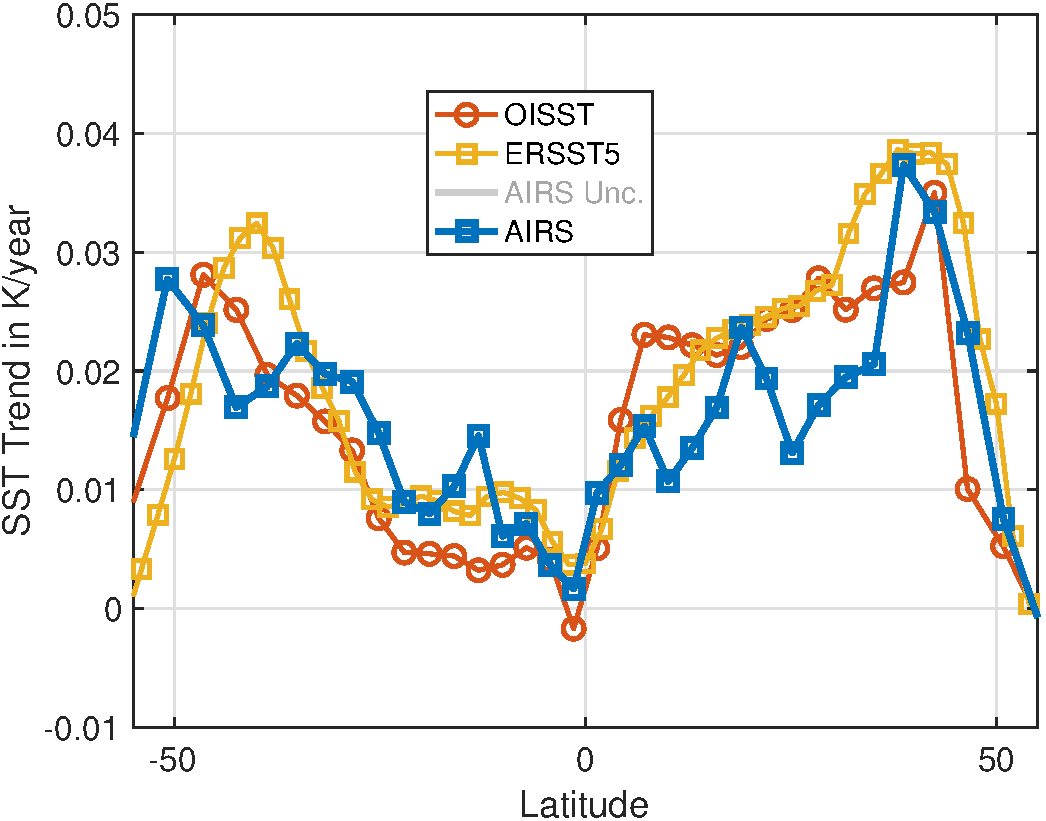
\includegraphics[width=0.7\linewidth]{./Figs/Pdf/zonal_sst_trends_12311_vs_oisst_ersst5_hottest_per_grid_envelope.pdf}
\end{center}
\end{frame}

\begin{frame}[label={sec:orgbc040fc}]{Pdf/new\_trend\_rand\_stats\_1231\_and\_2161\_era\_clr\_minus\_obs\_smoothed\_with\_2616\_labelled.pdf}
\begin{center}
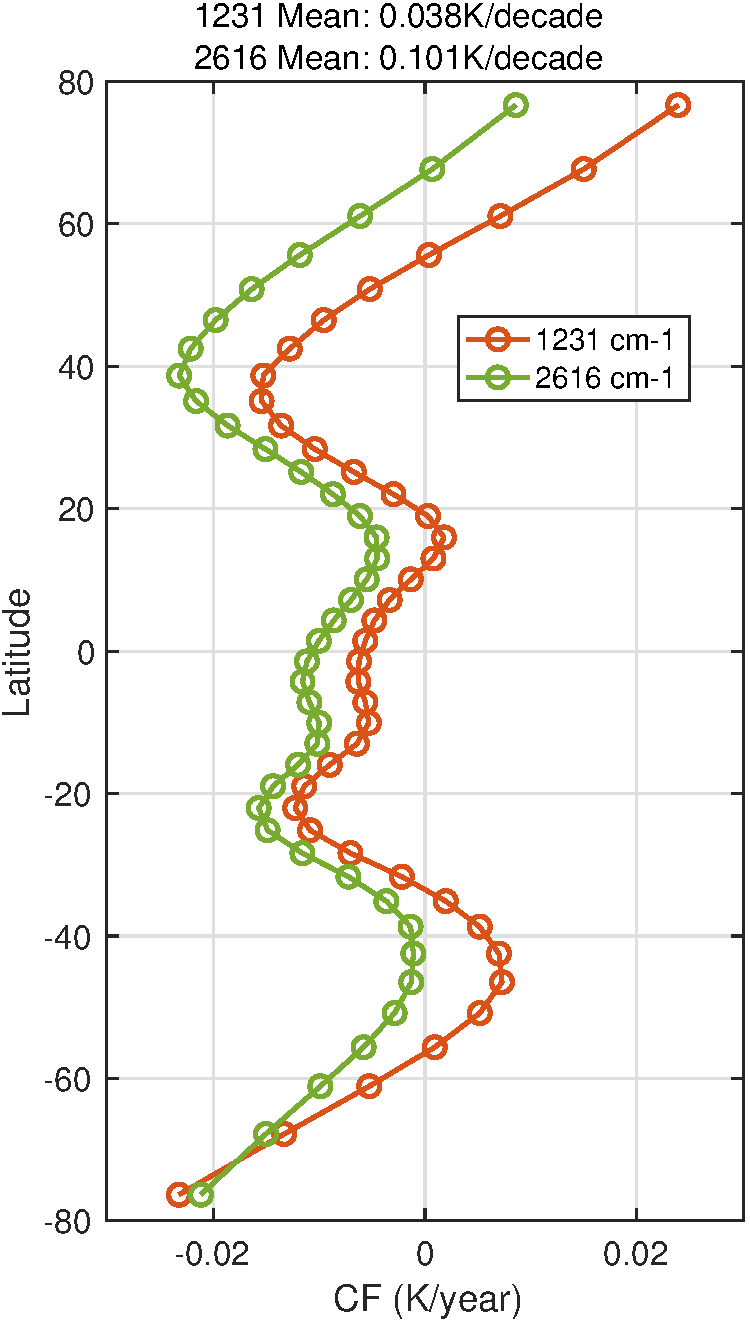
\includegraphics[width=0.7\linewidth]{./Figs/Pdf/new_trend_rand_stats_1231_and_2161_era_clr_minus_obs_smoothed_with_2616_labelled.pdf}
\end{center}
\end{frame}

\begin{frame}[label={sec:org72fd2fd}]{Pdf/new\_trend\_rand\_stats\_1231\_and\_2161\_era\_clr\_minus\_obs\_smoothed.pdf}
\begin{center}
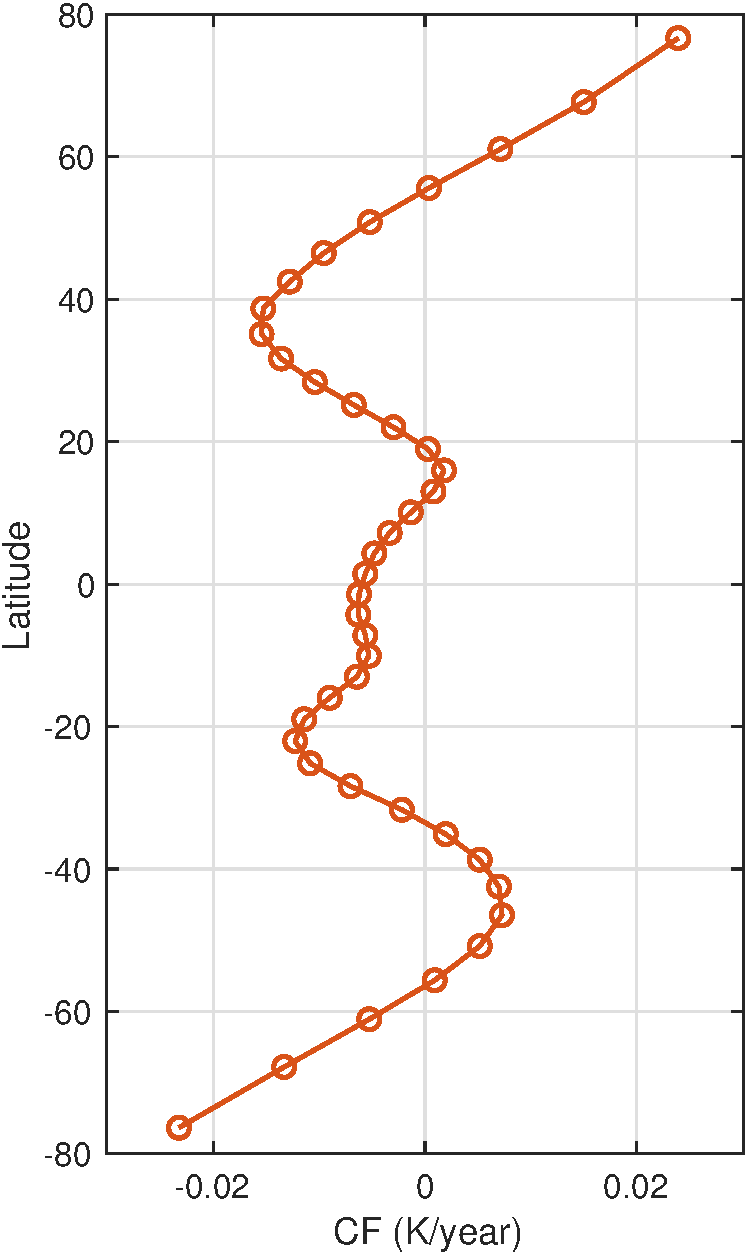
\includegraphics[width=0.7\linewidth]{./Figs/Pdf/new_trend_rand_stats_1231_and_2161_era_clr_minus_obs_smoothed.pdf}
\end{center}
\end{frame}

\begin{frame}[label={sec:org47ea8d3}]{new\_trend\_rand\_stats\_1231\_and\_2161\_era\_clr\_minus\_obs.pdf}
\begin{center}
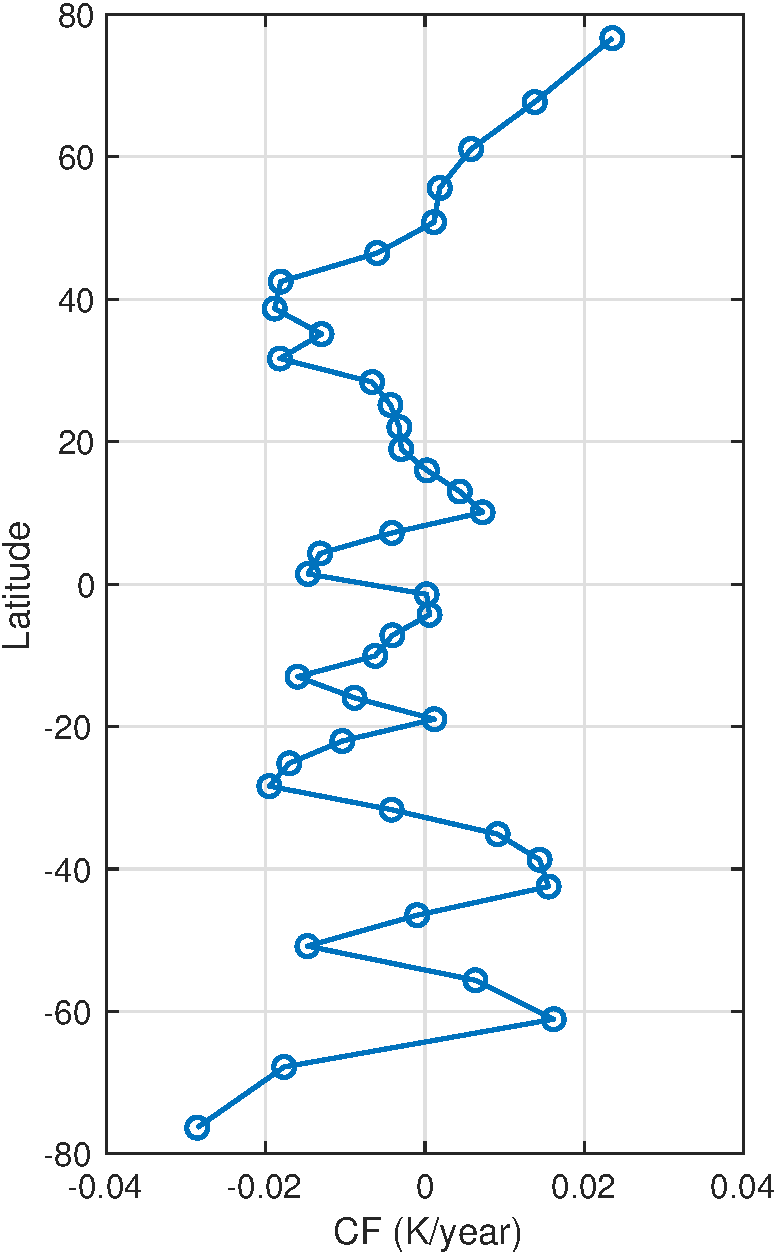
\includegraphics[width=0.7\linewidth]{./Figs/Pdf/new_trend_rand_stats_1231_and_2161_era_clr_minus_obs.pdf}
\end{center}
\end{frame}

\begin{frame}[label={sec:orgdf24683}]{Pdf/trenberth\_total\_only.pdf}
\begin{center}
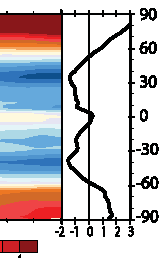
\includegraphics[width=0.7\linewidth]{./Figs/Pdf/trenberth_total_only.pdf}
\end{center}
\end{frame}

\begin{frame}[label={sec:orge689bc7}]{Pdf/trenberth2009\_clouds\_top.pdf}
\begin{center}
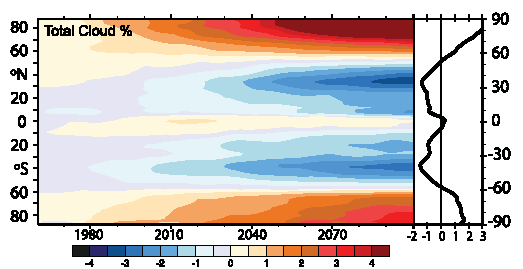
\includegraphics[width=0.7\linewidth]{./Figs/Pdf/trenberth2009_clouds_top.pdf}
\end{center}
\end{frame}

\begin{frame}[label={sec:org013b470}]{Pdf/trenberth2009\_clouds.pdf}
\begin{center}
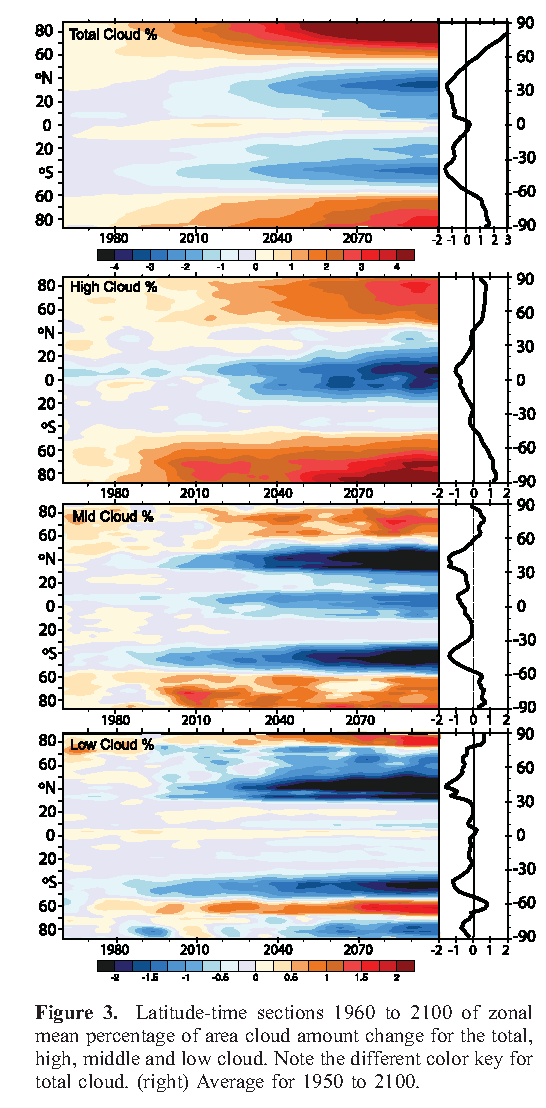
\includegraphics[width=0.7\linewidth]{./Figs/Pdf/trenberth2009_clouds.pdf}
\end{center}
\end{frame}

\begin{frame}[label={sec:org5555463}]{Pdf/lw\_h2o\_flux\_kernel.pdf}
\begin{center}
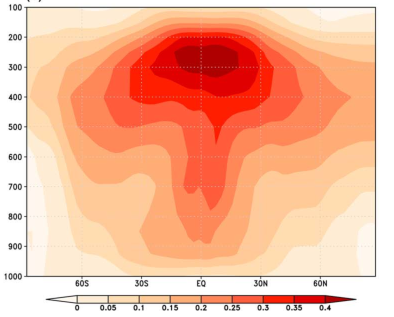
\includegraphics[width=0.7\linewidth]{./Figs/Pdf/lw_h2o_flux_kernel.pdf}
\end{center}
\end{frame}

\begin{frame}[label={sec:orga558808}]{Pdf/tseries\_sst\_obs\_global.pdf}
\begin{center}
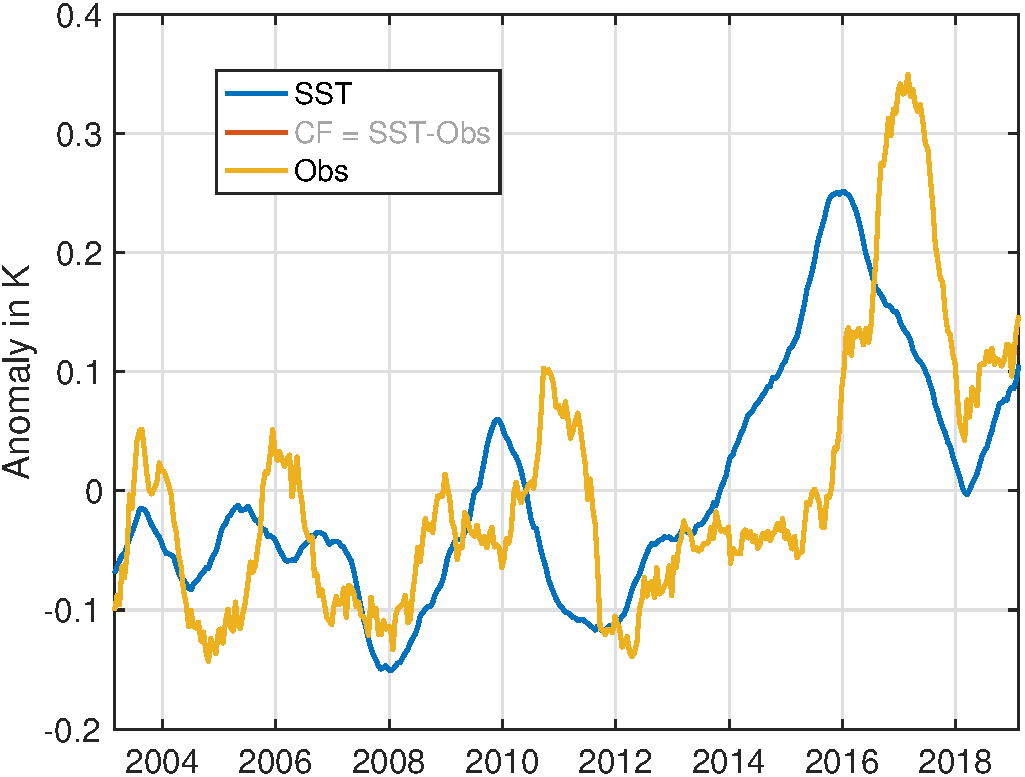
\includegraphics[width=0.7\linewidth]{./Figs/Pdf/tseries_sst_obs_global.pdf}
\end{center}
\end{frame}

\begin{frame}[label={sec:org352c195}]{Png/cf\_vs\_sst\_vs\_enso\_v2.png}
\begin{center}
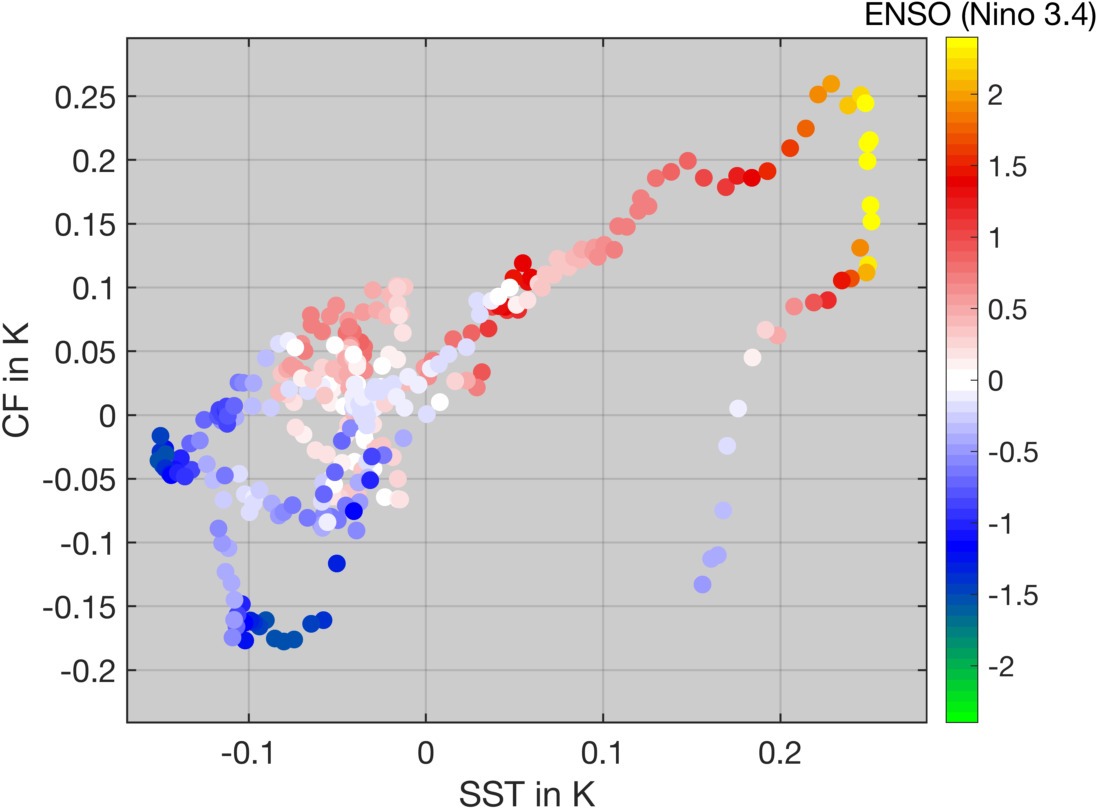
\includegraphics[width=0.7\linewidth]{./Figs/Png/cf_vs_sst_vs_enso_v2.png}
\end{center}
\end{frame}

\begin{frame}[label={sec:orgb25d076}]{Png/co2\_anom\_sst\_vs\_oisst\_clear\_sampled\_and\_era.png}
\begin{center}
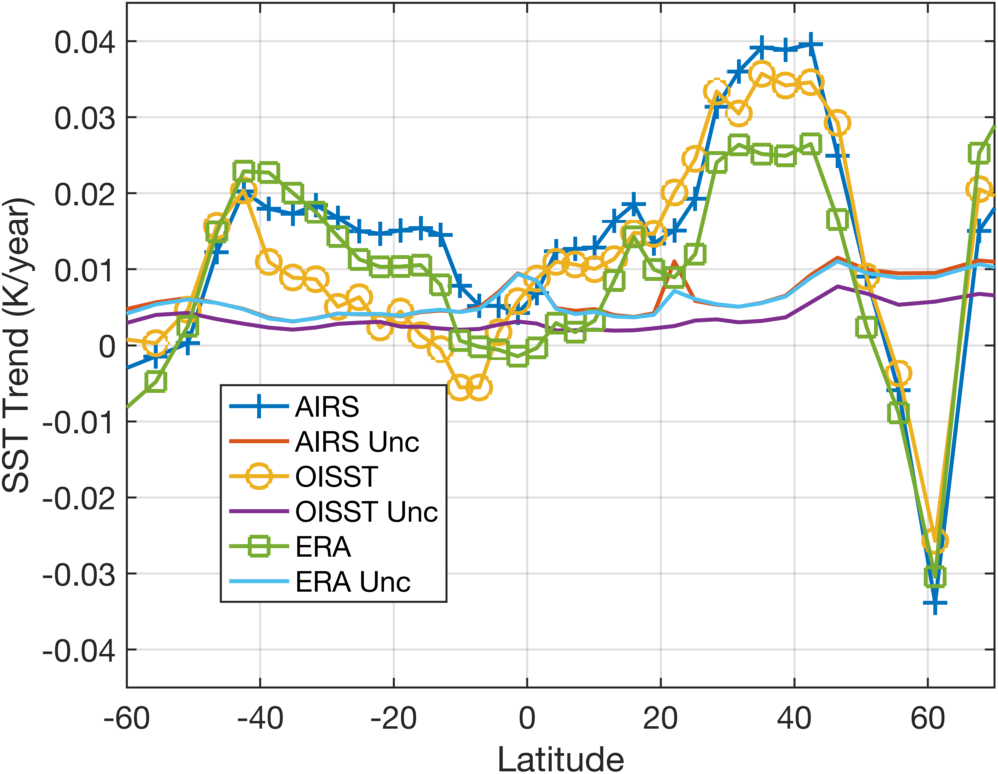
\includegraphics[width=0.7\linewidth]{./Figs/Png/co2_anom_sst_vs_oisst_clear_sampled_and_era.png}
\end{center}
\end{frame}

\begin{frame}[label={sec:orgb07954c}]{Png/co2\_anom\_sst\_vs\_oisst\_clear\_sampled.png}
\begin{center}
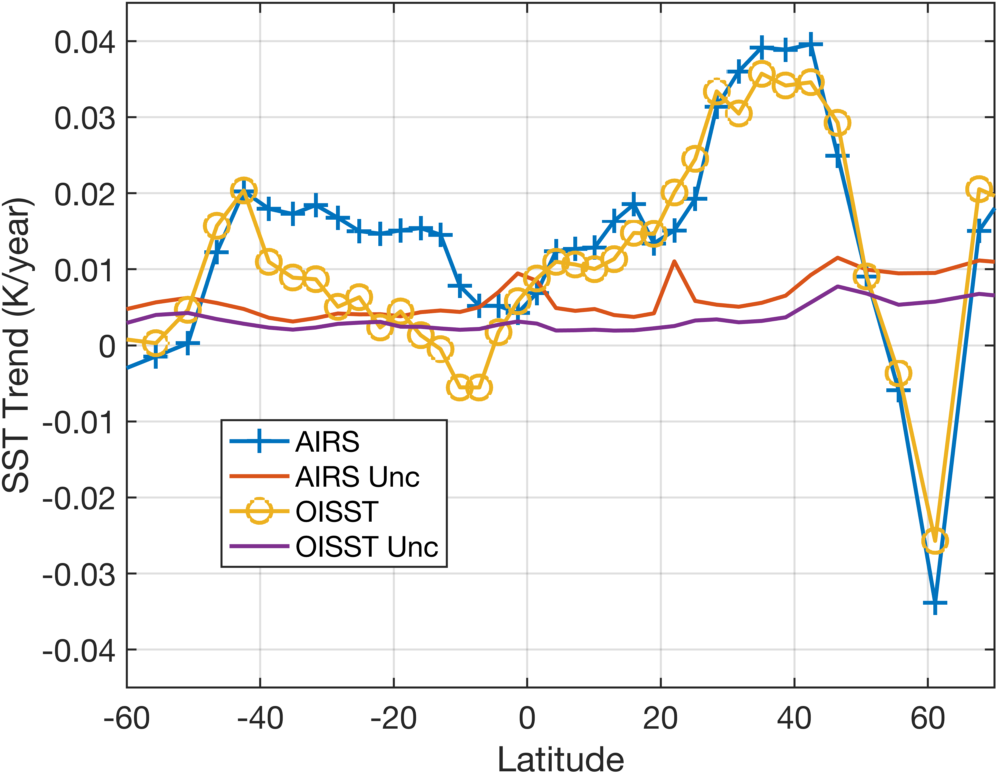
\includegraphics[width=0.7\linewidth]{./Figs/Png/co2_anom_sst_vs_oisst_clear_sampled.png}
\end{center}
\end{frame}

\begin{frame}[label={sec:org8b0cf7a}]{Png/oisst\_trend\_map.png}
\begin{center}
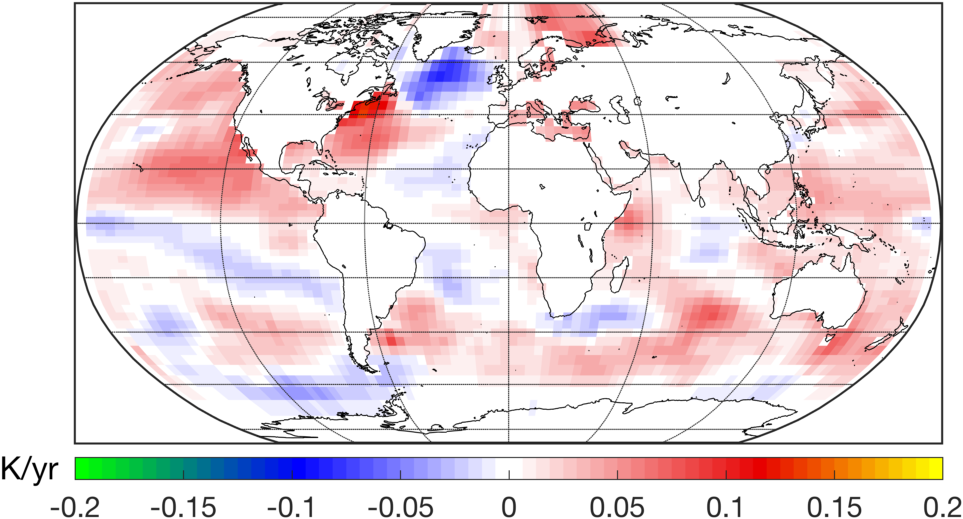
\includegraphics[width=0.7\linewidth]{./Figs/Png/oisst_trend_map.png}
\end{center}
\end{frame}

\begin{frame}[label={sec:orgf2e9184}]{Png/airs\_tsurf\_trend\_from\_1231cm\_trend.png}
\begin{center}
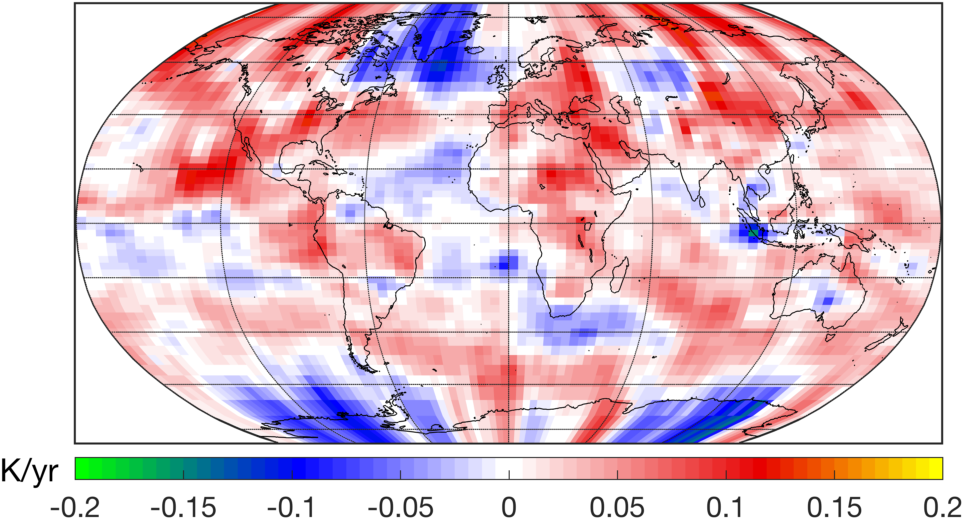
\includegraphics[width=0.7\linewidth]{./Figs/Png/airs_tsurf_trend_from_1231cm_trend.png}
\end{center}
\end{frame}

\begin{frame}[label={sec:org3b8b993}]{Png/era\_tsurf\_trend.png}
\begin{center}
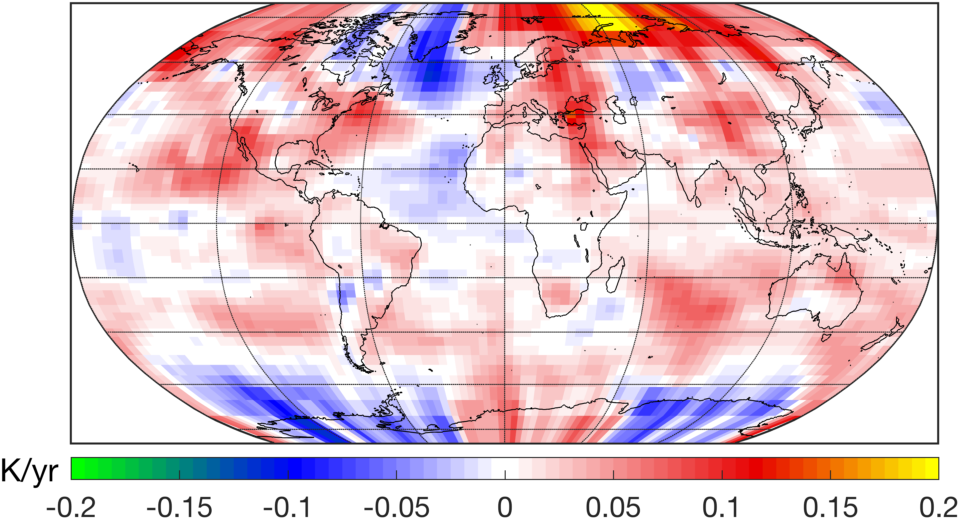
\includegraphics[width=0.7\linewidth]{./Figs/Png/era_tsurf_trend.png}
\end{center}
\end{frame}

\begin{frame}[label={sec:orgc766e8d}]{Pdf/ocean\_btobs\_delay\_from\_sst.pdf}
\begin{center}
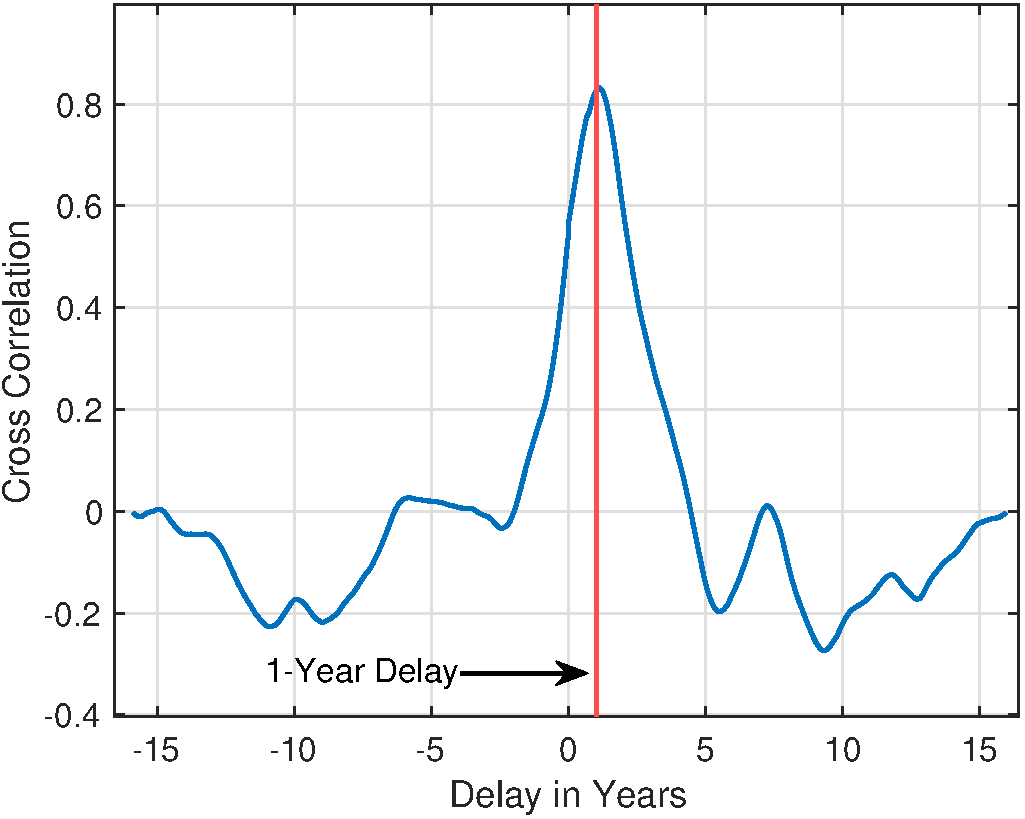
\includegraphics[width=0.7\linewidth]{./Figs/Pdf/ocean_btobs_delay_from_sst.pdf}
\end{center}
\end{frame}

\begin{frame}[label={sec:org21e05a4}]{Pdf/tseries\_sst\_cf\_obs\_global.pdf}
\begin{center}
\includegraphics[width=0.7\linewidth]{./Figs/Pdf/tseries_sst_cf_obs_global.pdf}
\end{center}
\end{frame}

\begin{frame}[label={sec:org8d3db40}]{Pdf/cf\_vs\_sst\_vs\_enso\_v2.pdf}
\begin{center}
\includegraphics[width=0.7\linewidth]{./Figs/Pdf/cf_vs_sst_vs_enso_v2.pdf}
\end{center}
\end{frame}

\begin{frame}[label={sec:orgd36355f}]{Pdf/cf\_vs\_sst\_vs\_year\_2019.pdf}
\begin{center}
\includegraphics[width=0.7\linewidth]{./Figs/Pdf/cf_vs_sst_vs_year_2019.pdf}
\end{center}
\end{frame}

\begin{frame}[label={sec:orga69d92d}]{Pdf/cf\_vs\_sst\_vs\_year\_2018.pdf}
\begin{center}
\includegraphics[width=0.7\linewidth]{./Figs/Pdf/cf_vs_sst_vs_year_2018.pdf}
\end{center}
\end{frame}

\begin{frame}[label={sec:org2f8728f}]{Pdf/cf\_vs\_sst\_vs\_year\_2017.pdf}
\begin{center}
\includegraphics[width=0.7\linewidth]{./Figs/Pdf/cf_vs_sst_vs_year_2017.pdf}
\end{center}
\end{frame}

\begin{frame}[label={sec:orga44157b}]{Pdf/cf\_vs\_sst\_vs\_year\_2016.pdf}
\begin{center}
\includegraphics[width=0.7\linewidth]{./Figs/Pdf/cf_vs_sst_vs_year_2016.pdf}
\end{center}
\end{frame}

\begin{frame}[label={sec:org3e4e3b1}]{Pdf/cf\_vs\_sst\_vs\_year\_2015.pdf}
\begin{center}
\includegraphics[width=0.7\linewidth]{./Figs/Pdf/cf_vs_sst_vs_year_2015.pdf}
\end{center}
\end{frame}

\begin{frame}[label={sec:orgc24c1df}]{Pdf/cf\_vs\_sst\_vs\_year\_2014.pdf}
\begin{center}
\includegraphics[width=0.7\linewidth]{./Figs/Pdf/cf_vs_sst_vs_year_2014.pdf}
\end{center}
\end{frame}

\begin{frame}[label={sec:orgd4bb1c1}]{Pdf/cf\_vs\_sst\_vs\_year\_2013.pdf}
\begin{center}
\includegraphics[width=0.7\linewidth]{./Figs/Pdf/cf_vs_sst_vs_year_2013.pdf}
\end{center}
\end{frame}

\begin{frame}[label={sec:orgabde611}]{Pdf/cf\_vs\_sst\_vs\_year\_2012.pdf}
\begin{center}
\includegraphics[width=0.7\linewidth]{./Figs/Pdf/cf_vs_sst_vs_year_2012.pdf}
\end{center}
\end{frame}

\begin{frame}[label={sec:org23bf21d}]{Pdf/cf\_vs\_sst\_vs\_year\_2011.pdf}
\begin{center}
\includegraphics[width=0.7\linewidth]{./Figs/Pdf/cf_vs_sst_vs_year_2011.pdf}
\end{center}
\end{frame}

\begin{frame}[label={sec:orgb363ce0}]{Pdf/cf\_vs\_sst\_vs\_year\_2010.pdf}
\begin{center}
\includegraphics[width=0.7\linewidth]{./Figs/Pdf/cf_vs_sst_vs_year_2010.pdf}
\end{center}
\end{frame}

\begin{frame}[label={sec:org4f03989}]{Pdf/cf\_vs\_sst\_vs\_year\_2009.pdf}
\begin{center}
\includegraphics[width=0.7\linewidth]{./Figs/Pdf/cf_vs_sst_vs_year_2009.pdf}
\end{center}
\end{frame}

\begin{frame}[label={sec:org86aec36}]{Pdf/cf\_vs\_sst\_vs\_year\_2008.pdf}
\begin{center}
\includegraphics[width=0.7\linewidth]{./Figs/Pdf/cf_vs_sst_vs_year_2008.pdf}
\end{center}
\end{frame}

\begin{frame}[label={sec:orgf3c77e4}]{Pdf/cf\_vs\_sst\_vs\_year\_2007.pdf}
\begin{center}
\includegraphics[width=0.7\linewidth]{./Figs/Pdf/cf_vs_sst_vs_year_2007.pdf}
\end{center}
\end{frame}

\begin{frame}[label={sec:org736fb9f}]{Pdf/cf\_vs\_sst\_vs\_year\_2006.pdf}
\begin{center}
\includegraphics[width=0.7\linewidth]{./Figs/Pdf/cf_vs_sst_vs_year_2006.pdf}
\end{center}
\end{frame}

\begin{frame}[label={sec:org9472fd3}]{Pdf/cf\_vs\_sst\_vs\_year\_2005.pdf}
\begin{center}
\includegraphics[width=0.7\linewidth]{./Figs/Pdf/cf_vs_sst_vs_year_2005.pdf}
\end{center}
\end{frame}

\begin{frame}[label={sec:org80dae69}]{Pdf/cf\_vs\_sst\_vs\_year\_2004.pdf}
\begin{center}
\includegraphics[width=0.7\linewidth]{./Figs/Pdf/cf_vs_sst_vs_year_2004.pdf}
\end{center}
\end{frame}

\begin{frame}[label={sec:org2ec9343}]{Pdf/cf\_vs\_sst\_vs\_year\_2003.pdf}
\begin{center}
\includegraphics[width=0.7\linewidth]{./Figs/Pdf/cf_vs_sst_vs_year_2003.pdf}
\end{center}
\end{frame}

\begin{frame}[label={sec:org599094e}]{Pdf/tseries\_sst\_cf\_obs\_global.pdf}
\begin{center}
\includegraphics[width=0.7\linewidth]{./Figs/Pdf/tseries_sst_cf_obs_global.pdf}
\end{center}
\end{frame}

\begin{frame}[label={sec:org2e2c62a}]{Png/water\_chans\_1400to1600\_trend\_vs\_btobs\_2dhist\_global.png}
\begin{center}
\includegraphics[width=0.7\linewidth]{./Figs/Png/water_chans_1400to1600_trend_vs_btobs_2dhist_global.png}
\end{center}
\end{frame}
\end{document}